\documentclass[a4paper, 12pt]{article}

\usepackage{geometry} % Простой способ задавать поля
\geometry{top=25mm}
\geometry{bottom=25mm}
\geometry{left=30mm}
\geometry{right=20mm}

\usepackage{cmap}                
\usepackage{mathtext}         
\usepackage[T2A]{fontenc}
\usepackage[utf8]{inputenc}    
\usepackage[british]{babel}	
\usepackage{tablefootnote}
\usepackage{threeparttable}
\usepackage{threeparttablex}

\usepackage{geometry} % Простой способ задавать поля
\geometry{top=25mm}
\geometry{bottom=25mm}
\geometry{left=35mm}
\geometry{right=20mm}
\usepackage{setspace}
\usepackage[section]{placeins}

\usepackage{amsmath}
\usepackage{euscript}     % Шрифт Евклид
\usepackage{mathrsfs} % Красивый
%матшрифт

\usepackage{lscape}

%%% Работа с картинками
\usepackage{graphicx}  % Для вставки
%рисунков
\graphicspath{img/}  %
%папки с картинками
\setlength\fboxsep{3pt} % Отступ рамки
%\fbox{} от рисунка
\setlength\fboxrule{1pt} % Толщина линий
%рамки \fbox{}
%\usepackage{wrapfig} % Обтекание
%рисунков и таблиц текстом
\usepackage{grffile}

\usepackage{csquotes}
\usepackage[style=apa, sorting=nty, bibencoding=utf8]{biblatex}
\addbibresource{citations.bib}
\DeclareLanguageMapping{british}{british-apa}
\onehalfspacing

\usepackage{hyperref}

\title{Poverty, inequality and dictatorship}
\author{Vladimir Novikov}

\begin{document}

\maketitle

\begin{center}
    \subsection*{Abstract}

    \textit{This paper examines the relationship between the people's poverty and the political regime in a country. Using statistical modeling on a longitudinal data set I found that the extreme poverty is negatively associated with democracy, the relationship between the poverty and democracy could be described as a quadratic and varies with the level of poverty and interaction between poverty and income inequality provides contradictory results.}
    
\end{center}

\section{Introduction and problem statement}

\noindent This paper aims to contribute to the complex studies of the relationship between the socio-economic structure of the society and the political regime. I work in the mainstream political economy framework, assuming that the political institutions are the product of the interaction of the different groups within the society \parencite{inst_per, why_fail}. Precisely, I concentrate on a very specific group -- the poor, or people in poverty. There are numerous studies showing that the middle class is necessary for the democracy from the classical \textit{<<no bourgeois, no democracy>>} \parencite{social_origins} to more recent papers \parencite{econ_origins, corridor}. But why the poor do not fit the democracy? The \textbf{puzzle} is that while the poor are the main <<losers>> of the dictatorship \parencite{political_roots}, they appear to be the guardians and the main supporters of it \parencite{voting_for_autocracy}. Existing literature supposes various interpretations of such phenomenon, which I will shortly examine below, highlighting the main challenges which are yet to be studied.
	\\\\
	\noindent I will start this short survey from the individual level theories. There is evidence, that the chronicle poverty affects people's decision making: they prefer short term consumption to the detriment of the long-run benefits \parencite{poverty_consequences}. Also, such people tend to be risk-averse \parencite{poverty_risk} and have a lower level of trust \parencite{trust_poverty} and in general, are associated with fewer social capital \parencite{poverty_capital3}. Taking into account the evidence above, we can assume that poverty hinders collective action and cooperation. And as the large corpus of the social capital literature suggests the democratic institutions must work the right way \parencite{bowling, social_capital_democracy}. Finally, it is important to mention that not just the absolute poverty, but also the relative one is important, as high levels of inequality are also associated with the individual level demand for authoritarianism \parencite{relative_power}, however, the relationship is ambiguous \parencite{inequality_regimes, regimes_inequality}.  
	\\\\
	Moving to the nations and states level theories, the framework is defined by the classical Olson's study \parencite{regime_development} with the assumption that democracy can cause long term development and dictatorship can not. From another point of view, democracy and development seem to sustain each other \parencite{democracy_development}. On the opposite side of the spectrum, dictatorship and poverty are also appear to be in a beautiful friendship. As the so-called economic logic of autocracy makes the poor even poorer (while the elites get richer) \parencite{handbook}. As it was mentioned above, the poor are less likely to cooperate and oppose the regime, however, they are more likely to be co-opted \parencite{three_pilars, toolkit}. So to get various prizes for the electoral (and not only) support, the poor are the ones who falsify the elections and contribute to the authoritarian persistence \parencite{more_than_win}.
	
	\section{Hypotheses}
	
	As one can clearly see, previous papers provide a considerable amount of hypotheses ob the initial puzzle. Nonetheless, the frameworks lack the general theory on the interplay between poverty and dictatorship. That is why such a study is relevant nowadays as the existing literature suffers from a lack of either proper empirical investigations and pay too much attention to the role of the middle class or were held long ago on the potentially outdated data. The \textbf{subject} of the paper is the the authoritarian regimes survival. To fill in the lacuna in the existing theories, the main\textbf{ research question} is the following:
    \begin{quote}
    \textit{How people's poverty related with the non-democratic political regimes?}
    \end{quote}
    \noindent With a focus on a causal mechanism of the relationship. Thus I propose several \textbf{hypotheses}. As the null hypothesis it might be tested whether:
    \begin{quote}
        \textit{Hypothesis 1: The people's poverty is associated with the less democratic political regime.}   
    \end{quote}
    Przeworski's study suggests that there might be non-linear relationship between the people's income and the political regime. Authoritarian survival is associated with either very low (GDP per capita below \$ 1000) or very high (per capita GDP above \$ 7000) income \parencite{democracy_development}. And thus the second hypothesis of the paper is the following:
    \begin{quote}
        \textit{Hypothesis 2: The relationship between the people's poverty and the political regime might be non-linear and follows reversed U-shape.}    
    \end{quote}
    An alternative explanation, suggested by the literature, might be the relative, not only than absolute poverty, i.e. combination of the poverty and inequality. To test it I propose the third hypotheses:
    \begin{quote}
        \textit{Hypothesis 3: Interaction between the poverty and the income inequality strengthens the relation with the dictatorship.}
    \end{quote}
    
    \section{Data}
    
        \begin{table}[!htbp] \centering 
  \caption{Descriptive Statistics} 
  \label{descr} 
  \resizebox{\columnwidth}{!}{%
\begin{tabular}{@{\extracolsep{5pt}}lccccccc} 
\\[-1.8ex]\hline 
\hline \\[-1.8ex] 
Statistic & \multicolumn{1}{c}{N} & \multicolumn{1}{c}{Mean} & \multicolumn{1}{c}{St. Dev.} & \multicolumn{1}{c}{Min} & \multicolumn{1}{c}{Pctl(25)} & \multicolumn{1}{c}{Pctl(75)} & \multicolumn{1}{c}{Max} \\ 
\hline \\[-1.8ex] 
e\_polity2 & 8,710 & 0.980 & 7.408 & $-$10.000 & $-$7.000 & 8.000 & 10.000 \\ 
poverty\_nat & 787 & 28.682 & 16.272 & 0.400 & 16.900 & 38.250 & 83.300 \\ 
poverty19 & 1,690 & 10.429 & 17.762 & 0.000 & 0.300 & 11.700 & 94.100 \\ 
poverty32 & 1,690 & 19.949 & 25.967 & 0.000 & 0.700 & 30.375 & 98.500 \\ 
poverty55 & 1,690 & 33.107 & 32.425 & 0.000 & 2.200 & 57.500 & 100.000 \\ 
poverty\_gap\_19 & 1,690 & 4.029 & 7.917 & 0.000 & 0.100 & 3.900 & 63.600 \\ 
poverty\_gap\_32 & 1,690 & 8.613 & 13.426 & 0.000 & 0.300 & 10.900 & 77.100 \\ 
poverty\_gap\_55 & 1,690 & 16.259 & 19.769 & 0.000 & 0.900 & 24.900 & 100.000 \\ 
v2x\_regime & 9,991 & 1.227 & 1.093 & 0.000 & 0.000 & 2.000 & 3.000 \\ 
e\_fh\_status & 7,597 & 1.971 & 0.816 & 1.000 & 1.000 & 3.000 & 3.000 \\ 
GDP\_pc\_ppp & 5,597 & 14,814.110 & 18,438.370 & 285.586 & 2,706.084 & 20,174.730 & 154,095.700 \\ 
population\_WB & 12,864 & 24,427,915.000 & 102,316,494.000 & 3,893.000 & 498,919.000 & 13,341,350.000 & 1,397,715,000.000 \\ 
v2regsupgroupssize & 8,853 & 0.600 & 1.112 & $-$2.948 & $-$0.256 & 1.571 & 2.594 \\ 
v2xeg\_eqdr & 10,013 & 0.555 & 0.289 & 0.014 & 0.293 & 0.829 & 0.987 \\ 
gini\_WB & 1,654 & 38.702 & 9.325 & 20.700 & 31.600 & 45.300 & 65.800 \\ 
regime & 7,068 & 0.544 & 5.190 & $-$7.531 & $-$5.208 & 5.815 & 6.978 \\ 
\hline \\[-1.8ex] 
\end{tabular} 
}
\end{table} 
    
    \noindent I construct a time-series cross-sectional dataset for 221 unique country units from 1960 to 2020, however the data mostly covers period after 1990. As the panel is unbalanced, it requires close attention as it can be a source of a potential selection bias. The reason is data availability for the developing countries, i.e. the data is missing not at random, which does not allow me to use linear interpolation to impute the missing data. Thus I would work with the unbalances panel keeping in mind potential bias in the data. The descriptive statistics for the data are in the  Table \ref{descr} above.  As a main predictor variable I use several poverty indicators, namely: the share of the population under the certain poverty line, either universal or national. National poverty line is defined as a half of the median household income of the total population. Universal poverty lines are \$ 1.9, \$ 3.2 and \$ 5.5 daily income or consumption and national poverty lines are calculated as the half of the median income in the given country. Besides, I use the the poverty gap index, which is also counted for different poverty lines. The poverty gap index is the ratio by which the mean income of the poor falls below the poverty line. All the indicators above are collected from the World Bank World Development Indicators \parencite{worldbank}. Despite the fact that all the poverty measurements are provided by the single agency, data on the national poverty lines is collected by the state statistical which might provide robustness to the results. The response variable -- the political regime is measured with the Polity IV estimate \parencite{polity}, which applies a scale from -10 to 10 to describe the spectre of the political regimes from full autocracy to full democracy. In the robustness section of the paper I also use the index including Polity IV, Varieties of Democracy \parencite{VDemV10} and Freedom House \parencite{freedomhouse} political regime estimates. 
    \\\\
    Income inequality is measured with the Gini index, collected by the World Bank. Considering all the critics, Gini remains the only universal and available for most country-year units estimate. As other control variables, I use GDP per capita PPP indicator and the population of a country in a given year, all measured by World Bank \parencite{worldbank}. Apart from that,  expert-coded indexes, measuring main regime support group size -- to control for co-optation by the regime and equality of the resources distribution and access to public services -- to control for redistribution are used as a control variables \parencite{VDemV10}.
    
    \section{Methods}
    
    To test the hypotheses, proposed above, I apply the following identification strategy: for each hypothesis set of different poverty estimates is used, as a first stage robustness check. Also I use lagged dependent variable (political regime) to partially address auto correlation issue, as the data contains many time periods. Also I use log of most of the variables to approximate them for the Normal distribution, and for the poverty measurements I use log(poverty measure + 1) to prevent taking log from 0. The distributions of the variables and correlation plots are in the Appendix.
    \\\\
    To deal with the panel structure of the data, I choose fixed effects models. There are several reasons for that. First, I am interested in two types of statistical inference: temporary variability in a given country, which allows me to measure time invariant differences between countries in a starting conditions and a general relationship between poverty and political regime in an average country in an average year (as i am working with as large as possible worldwide sample). For the first purpose I use models with fixed effects on countries, for the second two-ways fixed effects on both countries and years. Second, both poverty and political regimes show time related trends as well as control variables (see Figures \ref{pol}, \ref{pov} in the Appendix). This might lead to the biased estimates on the pooled data. Third, low p-value of the F-test for individual effects supposes using models with fixed effects rather than pooled regression. Still the results for the pooled models as a baseline are in the appendix. The random effects models were rejected after the Hausman test, as a p-value is low, the random effects model estimates might be biased and inconsistent thus I prefer fixed effects modeling.
    
    \section{Results}
 
    \begin{table}[!htbp] \centering 
  \caption{Hypothesis 1, two-ways fixed effects} 
  \label{h1t} 
    \resizebox{\columnwidth}{!}{%
\begin{tabular}{@{\extracolsep{5pt}}lccccccc} 
\\[-1.8ex]\hline 
\hline \\[-1.8ex] 
 & \multicolumn{7}{c}{\textit{Dependent variable:}} \\ 
\cline{2-8} 
\\[-1.8ex] & \multicolumn{7}{c}{polity2\_lag} \\ 
\\[-1.8ex] & (1) & (2) & (3) & (4) & (5) & (6) & (7)\\ 
\hline \\[-1.8ex] 
 poverty\_nat & $-$0.021 &  &  &  &  &  &  \\ 
  & (0.021) &  &  &  &  &  &  \\ 
  & & & & & & & \\ 
 log(poverty19 + 1) &  & $-$0.688$^{*}$ &  &  &  &  &  \\ 
  &  & (0.415) &  &  &  &  &  \\ 
  & & & & & & & \\ 
 log(poverty32 + 1) &  &  & 0.241 &  &  &  &  \\ 
  &  &  & (0.396) &  &  &  &  \\ 
  & & & & & & & \\ 
 log(poverty55 + 1) &  &  &  & 0.621$^{*}$ &  &  &  \\ 
  &  &  &  & (0.353) &  &  &  \\ 
  & & & & & & & \\ 
 log(poverty\_gap\_19 + 1) &  &  &  &  & $-$0.960$^{*}$ &  &  \\ 
  &  &  &  &  & (0.527) &  &  \\ 
  & & & & & & & \\ 
 log(poverty\_gap\_32 + 1) &  &  &  &  &  & $-$0.404 &  \\ 
  &  &  &  &  &  & (0.461) &  \\ 
  & & & & & & & \\ 
 log(poverty\_gap\_55 + 1) &  &  &  &  &  &  & 0.361 \\ 
  &  &  &  &  &  &  & (0.426) \\ 
  & & & & & & & \\ 
 log(GDP\_pc\_ppp) & $-$0.253 & $-$0.598 & 0.599 & 0.882 & $-$0.544 & $-$0.174 & 0.681 \\ 
  & (1.597) & (0.861) & (0.965) & (0.920) & (0.795) & (0.891) & (0.953) \\ 
  & & & & & & & \\ 
 log(population\_WB) & 4.234$^{*}$ & 3.907$^{**}$ & 4.166$^{***}$ & 3.826$^{**}$ & 3.309$^{**}$ & 4.141$^{***}$ & 4.147$^{***}$ \\ 
  & (2.353) & (1.517) & (1.504) & (1.494) & (1.549) & (1.521) & (1.505) \\ 
  & & & & & & & \\ 
 v2regsupgroupssize & 1.725$^{***}$ & 1.801$^{***}$ & 1.852$^{***}$ & 1.839$^{***}$ & 1.782$^{***}$ & 1.842$^{***}$ & 1.850$^{***}$ \\ 
  & (0.519) & (0.606) & (0.659) & (0.656) & (0.585) & (0.633) & (0.660) \\ 
  & & & & & & & \\ 
 v2xeg\_eqdr & 7.925$^{**}$ & 5.035 & 4.525 & 4.408 & 4.750 & 4.891 & 4.495 \\ 
  & (3.494) & (4.068) & (3.868) & (3.819) & (4.008) & (4.024) & (3.860) \\ 
  & & & & & & & \\ 
 log(gini\_WB) & $-$0.522 & 0.238 & $-$1.804 & $-$2.215 & 0.339 & $-$0.403 & $-$1.935 \\ 
  & (1.906) & (1.874) & (1.904) & (1.754) & (1.940) & (1.952) & (1.935) \\ 
  & & & & & & & \\ 
\hline \\[-1.8ex] 
Observations & 651 & 1,412 & 1,412 & 1,412 & 1,412 & 1,412 & 1,412 \\ 
R$^{2}$ & 0.155 & 0.149 & 0.138 & 0.144 & 0.156 & 0.140 & 0.139 \\ 
Adjusted R$^{2}$ & $-$0.086 & 0.026 & 0.014 & 0.020 & 0.034 & 0.016 & 0.015 \\ 
F Statistic & 15.431$^{***}$ (df = 6; 506) & 36.004$^{***}$ (df = 6; 1233) & 32.976$^{***}$ (df = 6; 1233) & 34.568$^{***}$ (df = 6; 1233) & 37.916$^{***}$ (df = 6; 1233) & 33.428$^{***}$ (df = 6; 1233) & 33.202$^{***}$ (df = 6; 1233) \\ 
\hline 
\hline \\[-1.8ex] 
\textit{Note: all the models use robust standard errors}  & \multicolumn{7}{r}{$^{*}$p$<$0.1; $^{**}$p$<$0.05; $^{***}$p$<$0.01} \\ 
\end{tabular} }
\end{table} 


    
    \subsection{First hypothesis}
    
    From the evidence in Table \ref{h1o} in the Appendix: the people's poverty is negative insignificant predictor for the low poverty lines (\$ 1.9 a day for the log of share of the population under the poverty line and \$ 1.9 and \$ 3.2 a day for log of the poverty gap). Relatively high poverty line of \$ 5.5 a day is indeed positively related with the democracy. Note that the HC1 type robust standard errors were used for all the results. P-value of the F-test for the two-ways fixed effects model gives no reason to prefer more complicated model. Nevertheless, for the robustness check the results could be achieved in the Table \ref{h1t}. There both the share of the population and the poverty gap under the \$ 1.9 a day poverty line are significant negative predictors of the democracy at the 10\% significance level. For the further robustness check, I re-estimated these two models on a truncated sample of the observations with the correlation between the response and the fitted value higher than 0.3. As the Table \ref{tranc} shows, coefficients for both poverty estimates remained negative, thus I can draw that both the share of the population and the poverty gap under \$ 1.9 a day poverty line are robust predictors of the dictatorship. For the higher poverty lines the first hypothesis should be rejected.

    \subsection{Second hypothesis: quadratic relationship}
    
    \begin{table}[!htbp] \centering 
  \caption{Hypothesis2, two-ways fixed-effects} 
  \label{h2t} 
  \resizebox{\columnwidth}{!}{%
\begin{tabular}{@{\extracolsep{5pt}}lccccccc} 
\\[-1.8ex]\hline 
\hline \\[-1.8ex] 
 & \multicolumn{7}{c}{\textit{Dependent variable:}} \\ 
\cline{2-8} 
\\[-1.8ex] & \multicolumn{7}{c}{polity2\_lag} \\ 
\\[-1.8ex] & (1) & (2) & (3) & (4) & (5) & (6) & (7)\\ 
\hline \\[-1.8ex] 
 poverty\_nat & 0.009 &  &  &  &  &  &  \\ 
  & (0.046) &  &  &  &  &  &  \\ 
  & & & & & & & \\ 
 I(poverty\_nat$\hat{\mkern6mu}$2) & $-$0.0004 &  &  &  &  &  &  \\ 
  & (0.001) &  &  &  &  &  &  \\ 
  & & & & & & & \\ 
 log(poverty19 + 1) &  & 0.797 &  &  &  &  &  \\ 
  &  & (0.711) &  &  &  &  &  \\ 
  & & & & & & & \\ 
 I(log(poverty19 + 1)$\hat{\mkern6mu}$2) &  & $-$0.392$^{*}$ &  &  &  &  &  \\ 
  &  & (0.214) &  &  &  &  &  \\ 
  & & & & & & & \\ 
 log(poverty32 + 1) &  &  & 1.681$^{**}$ &  &  &  &  \\ 
  &  &  & (0.726) &  &  &  &  \\ 
  & & & & & & & \\ 
 I(log(poverty32 + 1)$\hat{\mkern6mu}$2) &  &  & $-$0.373$^{**}$ &  &  &  &  \\ 
  &  &  & (0.163) &  &  &  &  \\ 
  & & & & & & & \\ 
 log(poverty55 + 1) &  &  &  & 0.878 &  &  &  \\ 
  &  &  &  & (0.667) &  &  &  \\ 
  & & & & & & & \\ 
 I(log(poverty55 + 1)$\hat{\mkern6mu}$2) &  &  &  & $-$0.055 &  &  &  \\ 
  &  &  &  & (0.159) &  &  &  \\ 
  & & & & & & & \\ 
 log(poverty\_gap\_19 + 1) &  &  &  &  & $-$0.715 &  &  \\ 
  &  &  &  &  & (0.623) &  &  \\ 
  & & & & & & & \\ 
 I(log(poverty\_gap\_19 + 1)$\hat{\mkern6mu}$2) &  &  &  &  & $-$0.081 &  &  \\ 
  &  &  &  &  & (0.221) &  &  \\ 
  & & & & & & & \\ 
 log(poverty\_gap\_32 + 1) &  &  &  &  &  & 1.490$^{*}$ &  \\ 
  &  &  &  &  &  & (0.810) &  \\ 
  & & & & & & & \\ 
 I(log(poverty\_gap\_32 + 1)$\hat{\mkern6mu}$2) &  &  &  &  &  & $-$0.539$^{**}$ &  \\ 
  &  &  &  &  &  & (0.244) &  \\ 
  & & & & & & & \\ 
 log(poverty\_gap\_55 + 1) &  &  &  &  &  &  & 1.921$^{**}$ \\ 
  &  &  &  &  &  &  & (0.797) \\ 
  & & & & & & & \\ 
 I(log(poverty\_gap\_55 + 1)$\hat{\mkern6mu}$2) &  &  &  &  &  &  & $-$0.414$^{**}$ \\ 
  &  &  &  &  &  &  & (0.198) \\ 
  & & & & & & & \\ 
 log(GDP\_pc\_ppp) & $-$0.140 & $-$0.533 & 0.202 & 0.820 & $-$0.514 & $-$0.201 & 0.305 \\ 
  & (1.633) & (0.870) & (0.969) & (0.977) & (0.786) & (0.899) & (0.978) \\ 
  & & & & & & & \\ 
 log(population\_WB) & 3.904$^{*}$ & 2.528 & 3.007$^{**}$ & 3.759$^{**}$ & 3.123$^{*}$ & 2.413 & 3.078$^{**}$ \\ 
  & (2.241) & (1.624) & (1.487) & (1.511) & (1.709) & (1.595) & (1.504) \\ 
  & & & & & & & \\ 
 v2regsupgroupssize & 1.721$^{***}$ & 1.734$^{***}$ & 1.794$^{***}$ & 1.842$^{***}$ & 1.778$^{***}$ & 1.752$^{***}$ & 1.815$^{***}$ \\ 
  & (0.513) & (0.552) & (0.607) & (0.655) & (0.580) & (0.569) & (0.618) \\ 
  & & & & & & & \\ 
 v2xeg\_eqdr & 8.122$^{**}$ & 4.679 & 4.401 & 4.470 & 4.756 & 4.531 & 4.567 \\ 
  & (3.467) & (3.902) & (3.917) & (3.885) & (3.989) & (3.855) & (3.927) \\ 
  & & & & & & & \\ 
 log(gini\_WB) & $-$0.517 & $-$0.639 & $-$1.856 & $-$2.148 & 0.288 & $-$1.151 & $-$1.723 \\ 
  & (1.938) & (1.460) & (1.764) & (1.776) & (1.850) & (1.617) & (1.835) \\ 
  & & & & & & & \\ 
\hline \\[-1.8ex] 
Observations & 651 & 1,412 & 1,412 & 1,412 & 1,412 & 1,412 & 1,412 \\ 
R$^{2}$ & 0.156 & 0.171 & 0.161 & 0.144 & 0.156 & 0.170 & 0.156 \\ 
Adjusted R$^{2}$ & $-$0.086 & 0.050 & 0.039 & 0.020 & 0.034 & 0.049 & 0.033 \\ 
F Statistic & 13.360$^{***}$ (df = 7; 505) & 36.268$^{***}$ (df = 7; 1232) & 33.657$^{***}$ (df = 7; 1232) & 29.674$^{***}$ (df = 7; 1232) & 32.591$^{***}$ (df = 7; 1232) & 36.005$^{***}$ (df = 7; 1232) & 32.486$^{***}$ (df = 7; 1232) \\ 
\hline 
\hline \\[-1.8ex] 
\textit{Note: all the models use robust standard errors}  & \multicolumn{7}{r}{$^{*}$p$<$0.1; $^{**}$p$<$0.05; $^{***}$p$<$0.01} \\ 
\end{tabular}
}
\end{table}
    
    \noindent To test the second hypothesis arguing non-linear relationship between the poverty and the political regime, I use quadratic term models. The results for the individual fixed effects model are in the Table \ref{h2o} and for the two-ways fixed effects model in the Table \ref{h2t}. Both sets of regressions show similar pattern of the reversed U-shape curve as the relationship between poverty and dictatorship changes as the poverty increases. It means that at lower levels of poverty, it's increase is associated with regime democratization, however after certain point the relationship changes and after that poverty is associated with the dictatorship. Plots of the margin effects for the models (Figure \ref{h2o_m}) are in the Appendix and show that the margin effects are significant, as the confidence intervals do not cover zero. Therefore there is no reason to reject the second hypothesis that the relationship between poverty and the political regimes follows quadratic curve.
    
    \subsection{Third hypothesis: joint effect}
    
    The first hypothesis requires using interaction term between poverty and the income inequality. Again, both individual and two-ways fixed effects models (Table \ref{h3o}, \ref{h3t}) show similar results, the increase in inequality (as higher value of Gini index corresponds to higher levels of inequality) strengthens the relationship between poverty and dictatorship. The margin effects (Figures \ref{h3o_m}, \ref{h3t_m}) also is significant as confidence intervals do not cover zero. However, it might lead to a contradictory conclusion that with the higher levels of inequality the relationship between poverty and political regimes changes so that poverty is associated with democracy. These results give no reason to approve the third hypothesis in the form it was stated above.   
    
    
    \begin{table}[!htbp] \centering 
  \caption{Hypothesis 3, two-ways fixed effects} 
  \label{h3t} 
  \resizebox{\columnwidth}{!}{%
\begin{tabular}{@{\extracolsep{5pt}}lccccccc} 
\\[-1.8ex]\hline 
\hline \\[-1.8ex] 
 & \multicolumn{7}{c}{\textit{Dependent variable:}} \\ 
\cline{2-8} 
\\[-1.8ex] & \multicolumn{7}{c}{polity2\_lag} \\ 
\\[-1.8ex] & (1) & (2) & (3) & (4) & (5) & (6) & (7)\\ 
\hline \\[-1.8ex] 
 poverty\_nat & $-$0.239$^{**}$ &  &  &  &  &  &  \\ 
  & (0.116) &  &  &  &  &  &  \\ 
  & & & & & & & \\ 
 log(poverty19 + 1) &  & $-$5.651$^{**}$ &  &  &  &  &  \\ 
  &  & (2.883) &  &  &  &  &  \\ 
  & & & & & & & \\ 
 log(poverty32 + 1) &  &  & $-$4.797$^{*}$ &  &  &  &  \\ 
  &  &  & (2.452) &  &  &  &  \\ 
  & & & & & & & \\ 
 log(poverty55 + 1) &  &  &  & $-$4.197$^{*}$ &  &  &  \\ 
  &  &  &  & (2.520) &  &  &  \\ 
  & & & & & & & \\ 
 log(poverty\_gap\_19 + 1) &  &  &  &  & $-$8.018$^{**}$ &  &  \\ 
  &  &  &  &  & (4.028) &  &  \\ 
  & & & & & & & \\ 
 log(poverty\_gap\_32 + 1) &  &  &  &  &  & $-$5.532$^{*}$ &  \\ 
  &  &  &  &  &  & (3.058) &  \\ 
  & & & & & & & \\ 
 log(poverty\_gap\_55 + 1) &  &  &  &  &  &  & $-$4.461$^{*}$ \\ 
  &  &  &  &  &  &  & (2.595) \\ 
  & & & & & & & \\ 
 log(GDP\_pc\_ppp) & $-$0.116 & $-$0.707 & 0.676 & 1.001 & $-$0.902 & $-$0.271 & 0.739 \\ 
  & (1.601) & (0.879) & (0.972) & (0.944) & (0.858) & (0.908) & (0.962) \\ 
  & & & & & & & \\ 
 log(population\_WB) & 5.352$^{**}$ & 4.583$^{***}$ & 4.851$^{***}$ & 4.234$^{***}$ & 3.894$^{**}$ & 4.838$^{***}$ & 4.756$^{***}$ \\ 
  & (2.651) & (1.547) & (1.545) & (1.494) & (1.534) & (1.572) & (1.546) \\ 
  & & & & & & & \\ 
 v2regsupgroupssize & 1.737$^{***}$ & 1.784$^{***}$ & 1.840$^{***}$ & 1.814$^{***}$ & 1.727$^{***}$ & 1.826$^{***}$ & 1.833$^{***}$ \\ 
  & (0.511) & (0.602) & (0.661) & (0.655) & (0.562) & (0.630) & (0.660) \\ 
  & & & & & & & \\ 
 v2xeg\_eqdr & 7.805$^{**}$ & 5.378 & 4.778 & 4.448 & 5.053 & 5.196 & 4.661 \\ 
  & (3.539) & (3.859) & (3.620) & (3.643) & (3.815) & (3.829) & (3.664) \\ 
  & & & & & & & \\ 
 log(gini\_WB) & $-$2.977 & $-$2.905 & $-$6.214$^{***}$ & $-$7.283$^{***}$ & $-$2.398 & $-$3.559$^{*}$ & $-$5.984$^{**}$ \\ 
  & (2.217) & (1.987) & (2.355) & (2.637) & (1.940) & (2.006) & (2.339) \\ 
  & & & & & & & \\ 
 poverty\_nat:log(gini\_WB) & 0.063$^{**}$ &  &  &  &  &  &  \\ 
  & (0.031) &  &  &  &  &  &  \\ 
  & & & & & & & \\ 
 log(poverty19 + 1):log(gini\_WB) &  & 1.392$^{*}$ &  &  &  &  &  \\ 
  &  & (0.751) &  &  &  &  &  \\ 
  & & & & & & & \\ 
 log(poverty32 + 1):log(gini\_WB) &  &  & 1.451$^{**}$ &  &  &  &  \\ 
  &  &  & (0.708) &  &  &  &  \\ 
  & & & & & & & \\ 
 log(poverty55 + 1):log(gini\_WB) &  &  &  & 1.403$^{*}$ &  &  &  \\ 
  &  &  &  & (0.760) &  &  &  \\ 
  & & & & & & & \\ 
 log(poverty\_gap\_19 + 1):log(gini\_WB) &  &  &  &  & 1.905$^{*}$ &  &  \\ 
  &  &  &  &  & (1.024) &  &  \\ 
  & & & & & & & \\ 
 log(poverty\_gap\_32 + 1):log(gini\_WB) &  &  &  &  &  & 1.438$^{*}$ &  \\ 
  &  &  &  &  &  & (0.801) &  \\ 
  & & & & & & & \\ 
 log(poverty\_gap\_55 + 1):log(gini\_WB) &  &  &  &  &  &  & 1.385$^{*}$ \\ 
  &  &  &  &  &  &  & (0.746) \\ 
  & & & & & & & \\ 
\hline \\[-1.8ex] 
Observations & 651 & 1,412 & 1,412 & 1,412 & 1,412 & 1,412 & 1,412 \\ 
R$^{2}$ & 0.162 & 0.160 & 0.149 & 0.152 & 0.171 & 0.150 & 0.147 \\ 
Adjusted R$^{2}$ & $-$0.079 & 0.038 & 0.026 & 0.028 & 0.050 & 0.026 & 0.023 \\ 
F Statistic & 13.941$^{***}$ (df = 7; 505) & 33.497$^{***}$ (df = 7; 1232) & 30.903$^{***}$ (df = 7; 1232) & 31.437$^{***}$ (df = 7; 1232) & 36.211$^{***}$ (df = 7; 1232) & 30.955$^{***}$ (df = 7; 1232) & 30.382$^{***}$ (df = 7; 1232) \\ 
\hline 
\hline \\[-1.8ex] 
\textit{Note: all the models use robust standard errors}  & \multicolumn{7}{r}{$^{*}$p$<$0.1; $^{**}$p$<$0.05; $^{***}$p$<$0.01} \\ 
\end{tabular}
}
\end{table}
    
    
    \section{Robustness}
    
    In this section I test the robustness of the models using the index, constructed with principal component analysis from Polity IV, Varieties of Democracy \parencite{VDemV10} and Freedom House \parencite{freedomhouse} political regime estimates as a response variable instead of the simple Polity IV score. I test the robustness of the two approved models from the first hypothesis (with \$ 1.9 poverty line) and all the models from the second hypothesis.
    \\\\
    \noindent The results for the models from the first hypothesis on a truncated sample with HC1 type robust standard errors are in the Table \ref{r1_t}. Coefficients before both predictors are  negative (yet insignificant), which allows to conclude that the extreme poverty is associated with less democratic regimes.
    
        \begin{table}[!htbp] \centering 
  \caption{Robust check, hypothesis 1, two-ways fixed effects, truncated sample} 
  \label{r1_t}
  \resizebox{\columnwidth}{!}{%
\begin{tabular}{@{\extracolsep{5pt}}lcc} 
\\[-1.8ex]\hline 
\hline \\[-1.8ex] 
 & \multicolumn{2}{c}{\textit{Dependent variable:}} \\ 
\cline{2-3} 
\\[-1.8ex] & \multicolumn{2}{c}{regime\_lag} \\ 
\\[-1.8ex] & (1) & (2)\\ 
\hline \\[-1.8ex] 
 log(poverty19 + 1) & $-$0.463 &  \\ 
  & (0.423) &  \\ 
  & & \\ 
 log(poverty\_gap\_19 + 1) &  & $-$0.844 \\ 
  &  & (0.522) \\ 
  & & \\ 
 log(GDP\_pc\_ppp) & 0.533 & 0.414 \\ 
  & (0.980) & (1.032) \\ 
  & & \\ 
 log(population\_WB) & 4.241$^{**}$ & 4.008$^{*}$ \\ 
  & (2.056) & (2.179) \\ 
  & & \\ 
 v2regsupgroupssize & 2.017$^{***}$ & 1.984$^{***}$ \\ 
  & (0.550) & (0.528) \\ 
  & & \\ 
 v2xeg\_eqdr & 5.062 & 3.922 \\ 
  & (4.035) & (3.881) \\ 
  & & \\ 
 log(gini\_WB) & 1.451 & 1.435 \\ 
  & (1.641) & (1.882) \\ 
  & & \\ 
\hline \\[-1.8ex] 
Observations & 644 & 607 \\ 
R$^{2}$ & 0.215 & 0.218 \\ 
Adjusted R$^{2}$ & 0.060 & 0.057 \\ 
F Statistic & 24.503$^{***}$ (df = 6; 537) & 23.325$^{***}$ (df = 6; 503) \\ 
\hline 
\hline \\[-1.8ex] 
\textit{Note: all the models use robust standard errors}  & \multicolumn{2}{r}{$^{*}$p$<$0.1; $^{**}$p$<$0.05; $^{***}$p$<$0.01} \\ 
\end{tabular} }
\end{table}
    
    
    \noindent Moving to the robust checks for the second hypothesis, I rerun the regression models with new index as a response variable. The results are available in the Tables \ref{r2o}, \ref{r2t} and are similar to the base models. However, the confidence intervals for the margin effects (Figures \ref{r2o_m}, \ref{r2t_m}) expanded, which makes the effect less significant and thus requires further checks with other indexes as a dependent variable.
    
      \begin{table}[!htbp] \centering 
  \caption{Robust check, hypothesis 2, two-ways fixed effects} 
  \label{r2t} 
  \resizebox{\columnwidth}{!}{%
\begin{tabular}{@{\extracolsep{5pt}}lccccccc} 
\\[-1.8ex]\hline 
\hline \\[-1.8ex] 
 & \multicolumn{7}{c}{\textit{Dependent variable:}} \\ 
\cline{2-8} 
\\[-1.8ex] & \multicolumn{7}{c}{regime\_lag} \\ 
\\[-1.8ex] & (1) & (2) & (3) & (4) & (5) & (6) & (7)\\ 
\hline \\[-1.8ex] 
 poverty\_nat & 0.012 &  &  &  &  &  &  \\ 
  & (0.036) &  &  &  &  &  &  \\ 
  & & & & & & & \\ 
 I(poverty\_nat$\hat{\mkern6mu}$2) & $-$0.0004 &  &  &  &  &  &  \\ 
  & (0.0004) &  &  &  &  &  &  \\ 
  & & & & & & & \\ 
 log(poverty19 + 1) &  & 0.587 &  &  &  &  &  \\ 
  &  & (0.486) &  &  &  &  &  \\ 
  & & & & & & & \\ 
 I(log(poverty19 + 1)$\hat{\mkern6mu}$2) &  & $-$0.280$^{**}$ &  &  &  &  &  \\ 
  &  & (0.141) &  &  &  &  &  \\ 
  & & & & & & & \\ 
 log(poverty32 + 1) &  &  & 1.185$^{**}$ &  &  &  &  \\ 
  &  &  & (0.502) &  &  &  &  \\ 
  & & & & & & & \\ 
 I(log(poverty32 + 1)$\hat{\mkern6mu}$2) &  &  & $-$0.260$^{**}$ &  &  &  &  \\ 
  &  &  & (0.106) &  &  &  &  \\ 
  & & & & & & & \\ 
 log(poverty55 + 1) &  &  &  & 0.664 &  &  &  \\ 
  &  &  &  & (0.449) &  &  &  \\ 
  & & & & & & & \\ 
 I(log(poverty55 + 1)$\hat{\mkern6mu}$2) &  &  &  & $-$0.047 &  &  &  \\ 
  &  &  &  & (0.108) &  &  &  \\ 
  & & & & & & & \\ 
 log(poverty\_gap\_19 + 1) &  &  &  &  & $-$0.489 &  &  \\ 
  &  &  &  &  & (0.412) &  &  \\ 
  & & & & & & & \\ 
 I(log(poverty\_gap\_19 + 1)$\hat{\mkern6mu}$2) &  &  &  &  & $-$0.071 &  &  \\ 
  &  &  &  &  & (0.148) &  &  \\ 
  & & & & & & & \\ 
 log(poverty\_gap\_32 + 1) &  &  &  &  &  & 1.045$^{*}$ &  \\ 
  &  &  &  &  &  & (0.560) &  \\ 
  & & & & & & & \\ 
 I(log(poverty\_gap\_32 + 1)$\hat{\mkern6mu}$2) &  &  &  &  &  & $-$0.379$^{**}$ &  \\ 
  &  &  &  &  &  & (0.162) &  \\ 
  & & & & & & & \\ 
 log(poverty\_gap\_55 + 1) &  &  &  &  &  &  & 1.371$^{**}$ \\ 
  &  &  &  &  &  &  & (0.535) \\ 
  & & & & & & & \\ 
 I(log(poverty\_gap\_55 + 1)$\hat{\mkern6mu}$2) &  &  &  &  &  &  & $-$0.295$^{**}$ \\ 
  &  &  &  &  &  &  & (0.128) \\ 
  & & & & & & & \\ 
 log(GDP\_pc\_ppp) & 0.080 & $-$0.359 & 0.159 & 0.578 & $-$0.377 & $-$0.140 & 0.216 \\ 
  & (1.170) & (0.584) & (0.663) & (0.674) & (0.531) & (0.607) & (0.670) \\ 
  & & & & & & & \\ 
 log(population\_WB) & 2.525 & 1.487 & 1.835$^{*}$ & 2.347$^{**}$ & 1.857$^{*}$ & 1.417 & 1.871$^{*}$ \\ 
  & (1.612) & (1.059) & (0.978) & (1.005) & (1.126) & (1.040) & (0.990) \\ 
  & & & & & & & \\ 
 v2regsupgroupssize & 1.070$^{***}$ & 1.065$^{***}$ & 1.107$^{***}$ & 1.141$^{***}$ & 1.093$^{***}$ & 1.077$^{***}$ & 1.121$^{***}$ \\ 
  & (0.379) & (0.371) & (0.408) & (0.441) & (0.388) & (0.383) & (0.415) \\ 
  & & & & & & & \\ 
 v2xeg\_eqdr & 5.755$^{**}$ & 3.697 & 3.504 & 3.564 & 3.762 & 3.603 & 3.626 \\ 
  & (2.283) & (2.643) & (2.648) & (2.615) & (2.697) & (2.614) & (2.654) \\ 
  & & & & & & & \\ 
 log(gini\_WB) & 0.071 & $-$0.253 & $-$1.100 & $-$1.287 & 0.464 & $-$0.580 & $-$0.988 \\ 
  & (1.375) & (0.970) & (1.171) & (1.175) & (1.240) & (1.070) & (1.212) \\ 
  & & & & & & & \\ 
\hline \\[-1.8ex] 
Observations & 651 & 1,412 & 1,412 & 1,412 & 1,412 & 1,412 & 1,412 \\ 
R$^{2}$ & 0.136 & 0.163 & 0.151 & 0.134 & 0.148 & 0.161 & 0.147 \\ 
Adjusted R$^{2}$ & $-$0.112 & 0.041 & 0.028 & 0.008 & 0.025 & 0.039 & 0.023 \\ 
F Statistic & 11.375$^{***}$ (df = 7; 505) & 34.178$^{***}$ (df = 7; 1232) & 31.281$^{***}$ (df = 7; 1232) & 27.150$^{***}$ (df = 7; 1232) & 30.645$^{***}$ (df = 7; 1232) & 33.825$^{***}$ (df = 7; 1232) & 30.213$^{***}$ (df = 7; 1232) \\ 
\hline 
\hline \\[-1.8ex] 
\textit{Note: all the models use robust standard errors}  & \multicolumn{7}{r}{$^{*}$p$<$0.1; $^{**}$p$<$0.05; $^{***}$p$<$0.01} \\ 
\end{tabular} 
}
\end{table}   
    
    \section{Discussion}
    
    In this section I review and reinterpret the results of the empirical analysis in the broader context. Starting with the findings of the paper, the first hypothesis that the poverty is associated with the less democratic regime was confirmed on the data but only for the extreme poverty (\$ 1.9 consumption daily) the result is robust. This result corresponds with the literature as the poorest people are the ones most vulnerable for the co-optation \parencite{voting_for_autocracy}. However, other paper suggest that the income shocks in poor countries lead to the democratization \parencite{rain_dem} so this topic requires further investigation. The second hypothesis, proposing quadratic relationship was confirmed as well, moreover the estimate is robust for using different response variable: the relationship between the people's poverty and the political regime follows reversed U-shapes curve. Or simply either low or high levels of poverty are associated with the dictatorship while medium is related with more democratic regimes.  It also corresponds with the existing studies in the field. Classic Przeworski's paper suspected  this sort of relationship \parencite{democracy_development}. Also this funding stands in line with the corpus of the middle class-democracy literature. Finally, the third hypothesis assuming the joint effect resulted into the surprising finding that with the higher levels of inequality poverty is positively correlated with democracy.
    \\\\
    Though, there are numerous limitations of this paper. There are at least two sources of endogeneity in the model. First, as it was mentioned above, there is a selection bias coming from the missing not at random data in the unbalanced panel. This could be resolved using other sources of the data and creating longitudinal dataset including data for more time periods. Second, there might be omitted variable bias as the models seem to be under specified (models fail to explain most of the variation of the response variable). While individual level factors and social capital were discussed in the literature survey in the beginning of the paper, they were not included in the model specifications due to the data availability issues. In addition to that, there is lack of exogenous predictors. Besides, the overall models' specifications can be improved by using first difference approach to describe the dynamics of the variables. Another way to improve the specification of the model is the binary defined political regime and the logistic regression.
    \\\\
    Despite the drawbacks, listed above, this paper provides some baseline evidence for the further and more detailed empirical investigation. At least, the analysis of the very recent data was provided at some points proving prior studies and at some (interaction between poverty and inequality) finding some unexpected relations.
    
    
\printbibliography


\section*{Appendix}
\FloatBarrier
\noindent Data, code and plots are also available \href{https://github.com/valdewastaken/MSA}{online}.

\begin{figure}
    \centering
    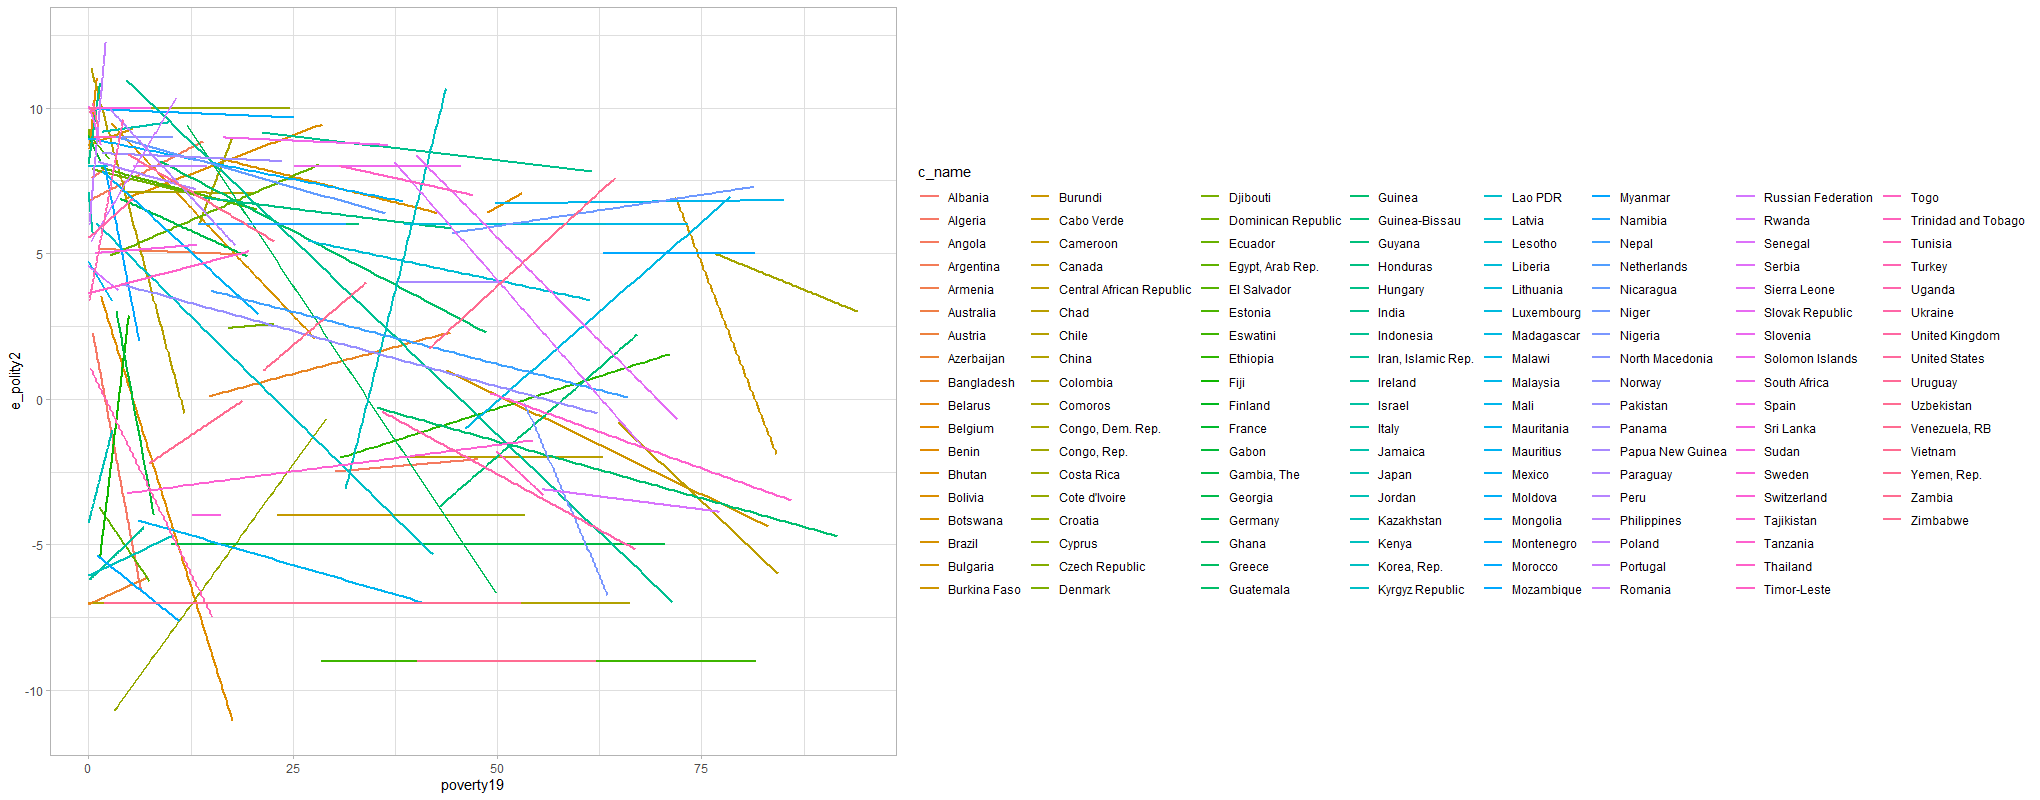
\includegraphics[width=\textwidth]{img/baseline.png}
    \caption{Country Trends, Regime and Poverty Relationship}
    \label{corr}
\end{figure}

\begin{figure}
    \centering
    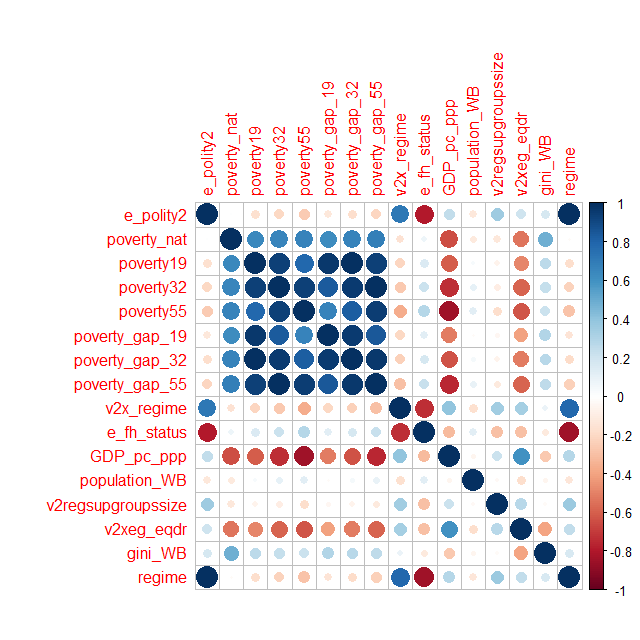
\includegraphics[width=\textwidth]{img/cor.png}
    \caption{Correlations}
    \label{corr}
\end{figure}


\begin{landscape}
\begin{figure}
    \centering
    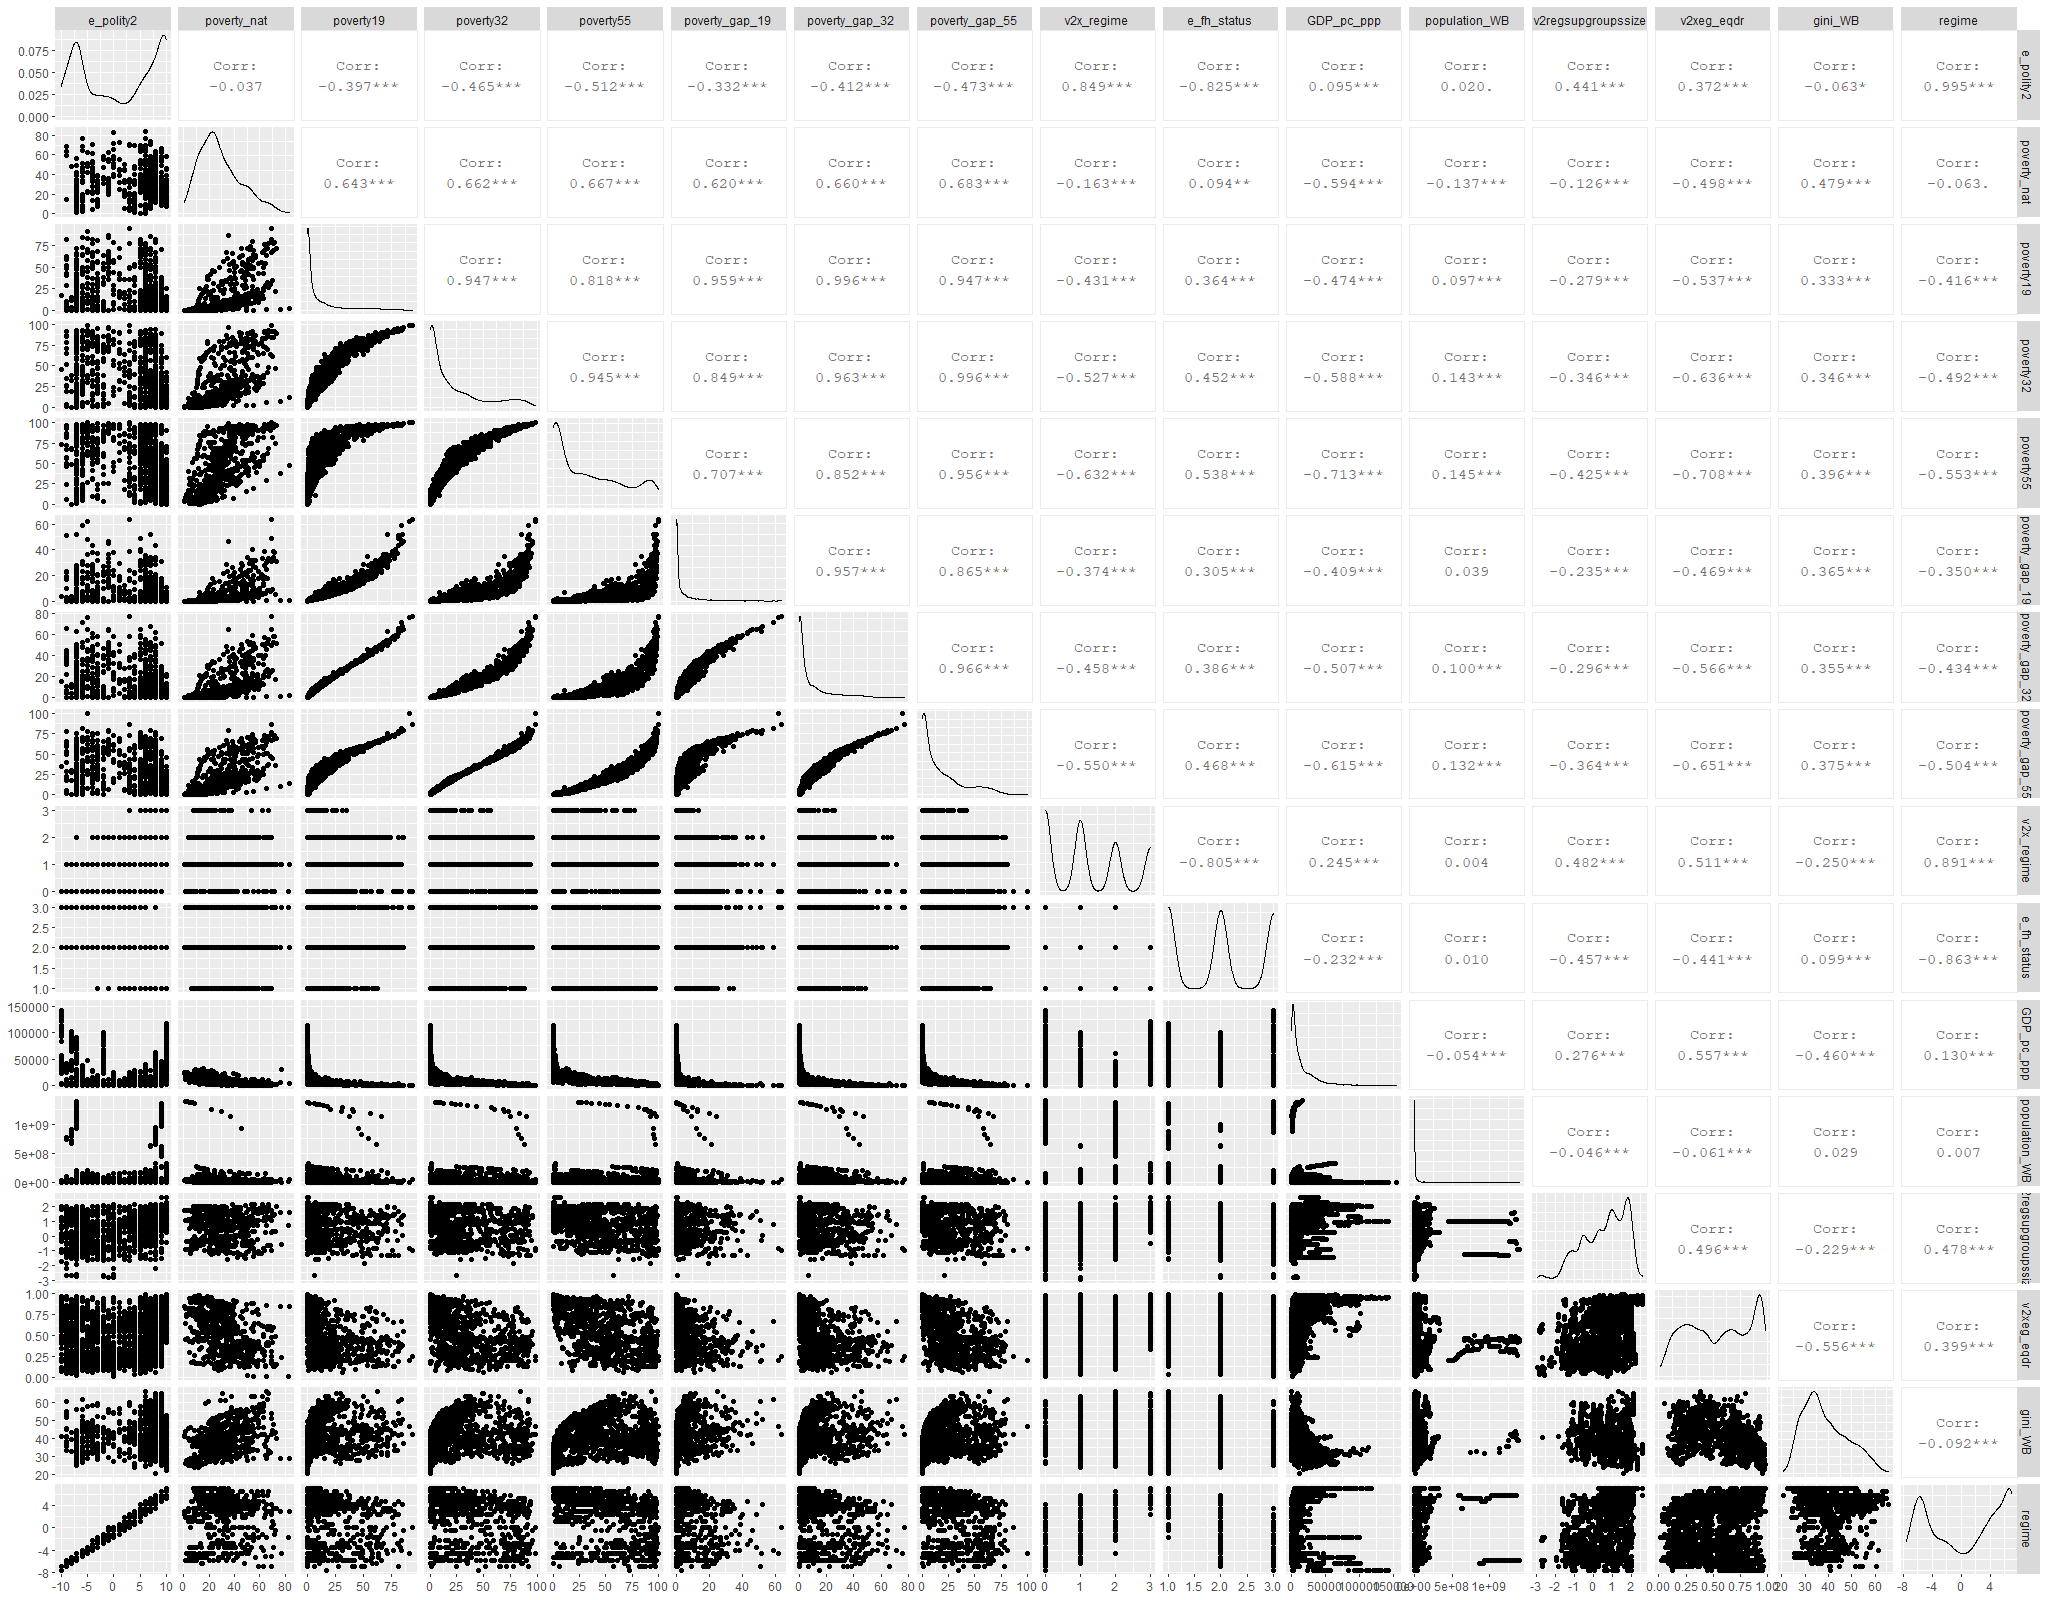
\includegraphics[width=20.5cm]{img/distributions.png}
    \caption{Variables Distributions}
    \label{distr}
\end{figure}
\end{landscape}

\begin{figure}
    \centering
    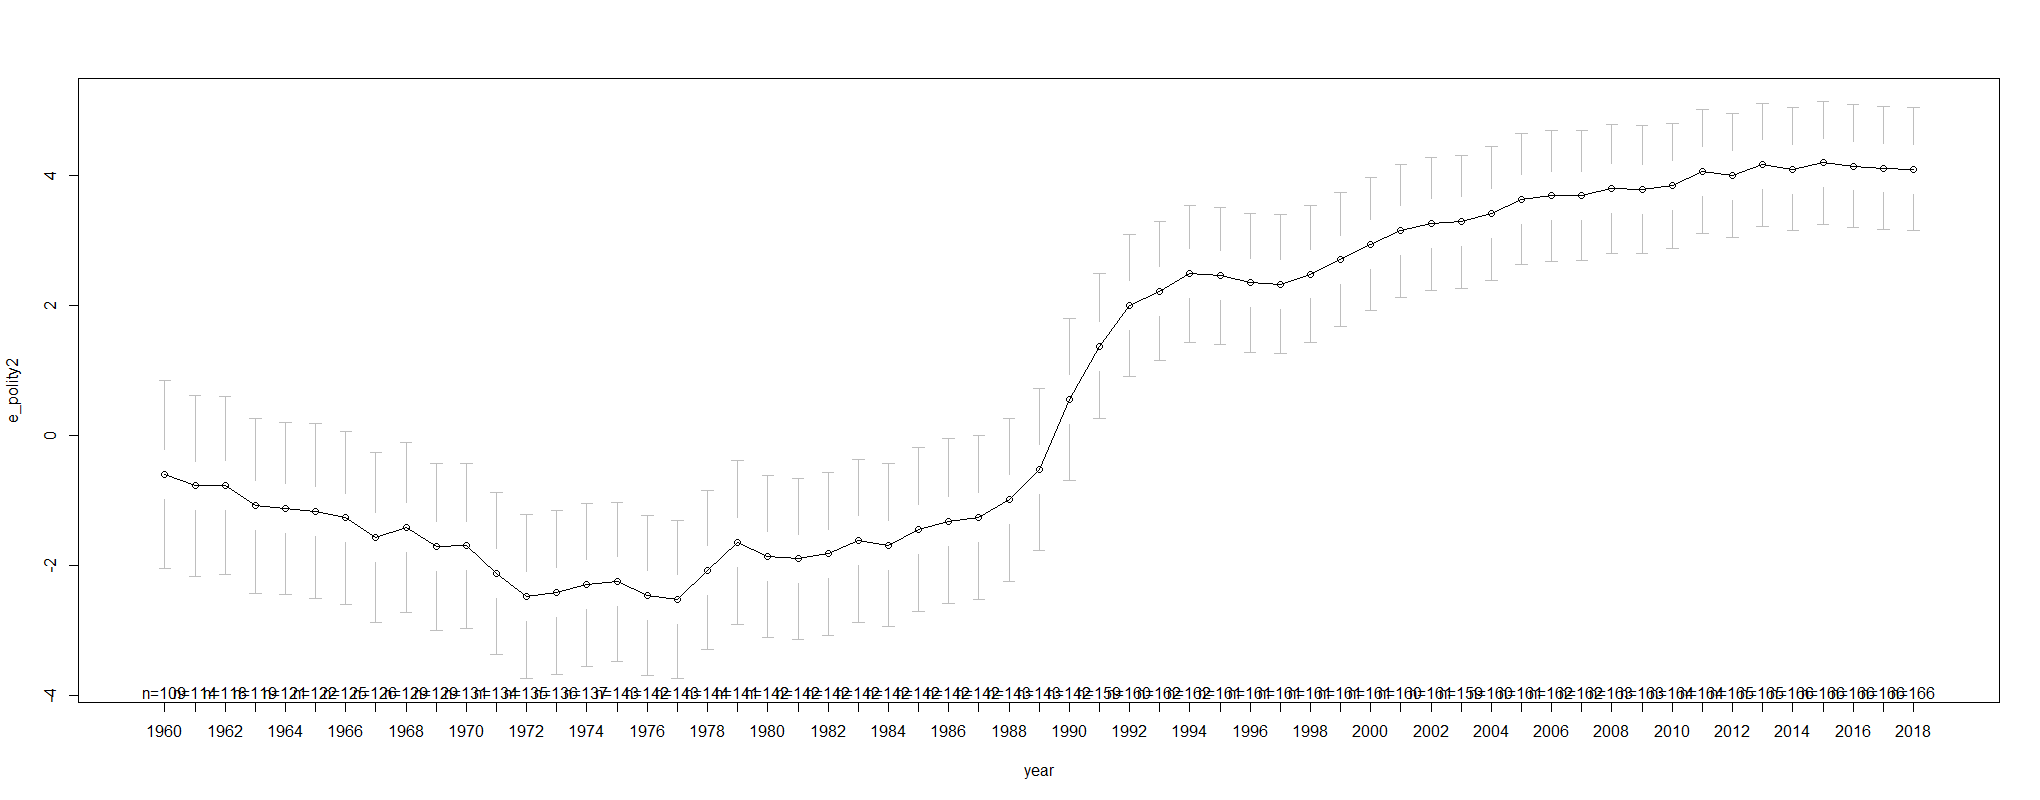
\includegraphics[width=\textwidth]{img/polity.png}
    \caption{Polity Dynamics}
    \label{pol}
\end{figure}

\begin{figure}
    \centering
    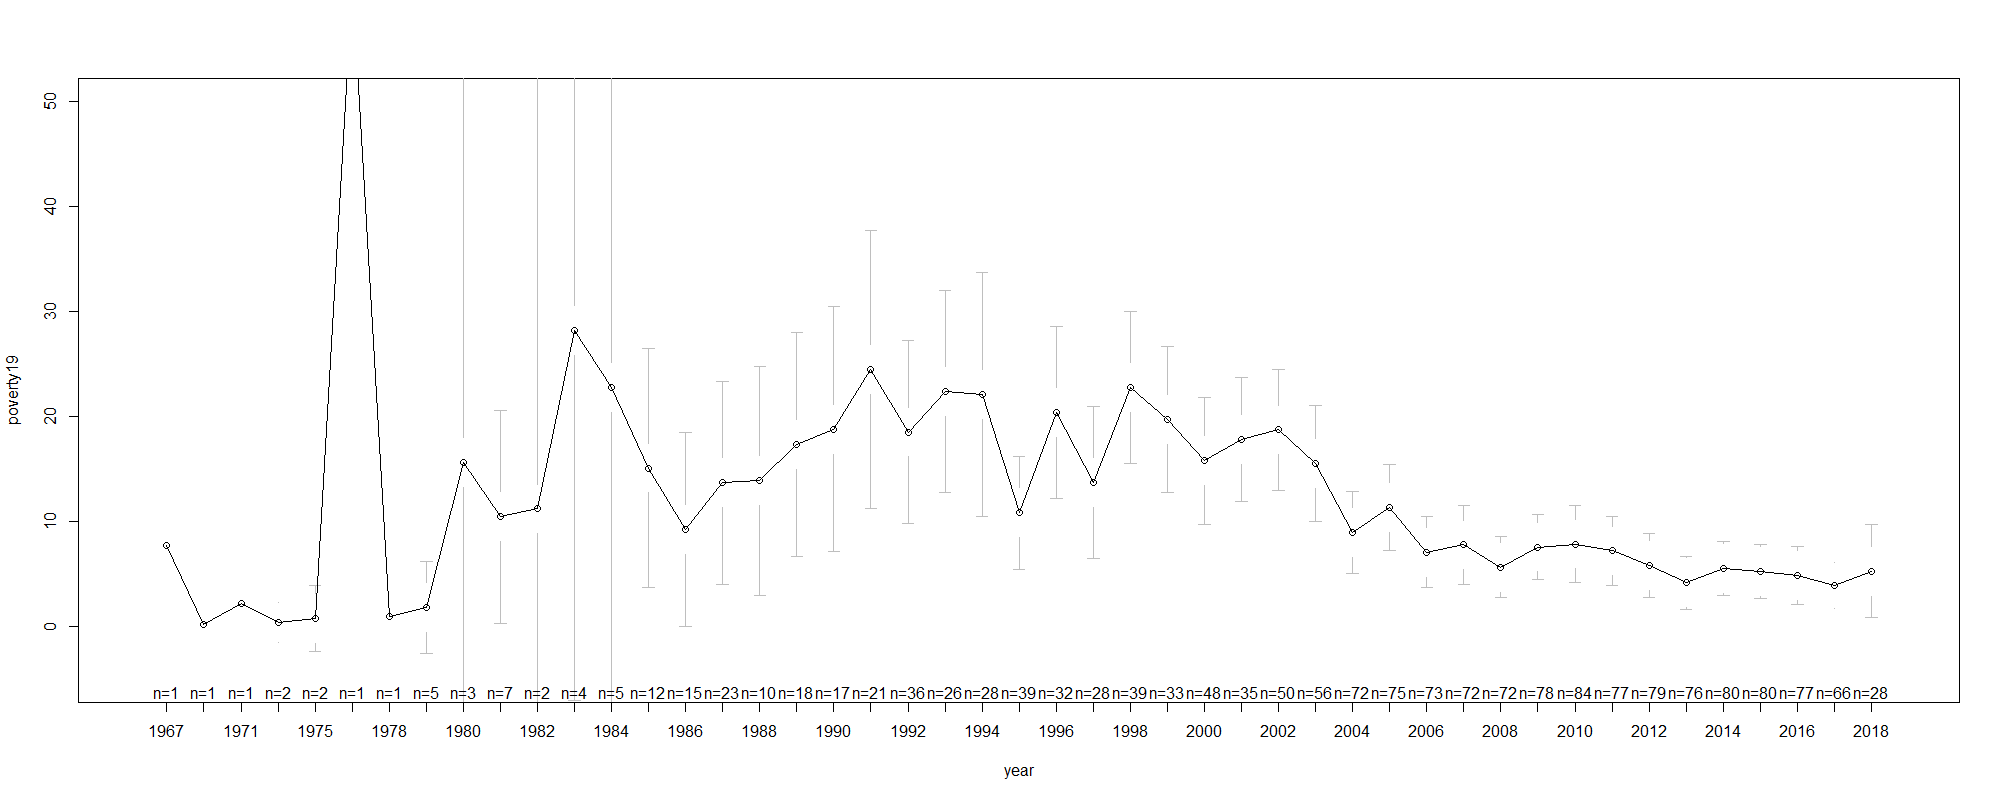
\includegraphics[width=\textwidth]{img/poverty.png}
    \caption{Poverty Dynamics}
    \label{pov}
\end{figure}


\begin{landscape}

\begin{table}[!htbp] \centering 
  \caption{Hypothesis 1, Pooled Models} 
  \label{pool} 
  \resizebox{\columnwidth}{!}{%
\begin{tabular}{@{\extracolsep{5pt}}lccccccc} 
\\[-1.8ex]\hline 
\hline \\[-1.8ex] 
 & \multicolumn{7}{c}{\textit{Dependent variable:}} \\ 
\cline{2-8} 
\\[-1.8ex] & \multicolumn{7}{c}{polity2\_lag} \\ 
\\[-1.8ex] & (1) & (2) & (3) & (4) & (5) & (6) & (7)\\ 
\hline \\[-1.8ex] 
 poverty\_nat & 0.074$^{**}$ &  &  &  &  &  &  \\ 
  & (0.030) &  &  &  &  &  &  \\ 
  & & & & & & & \\ 
 log(poverty19 + 1) &  & 0.112 &  &  &  &  &  \\ 
  &  & (0.518) &  &  &  &  &  \\ 
  & & & & & & & \\ 
 log(poverty32 + 1) &  &  & $-$0.234 &  &  &  &  \\ 
  &  &  & (0.465) &  &  &  &  \\ 
  & & & & & & & \\ 
 log(poverty55 + 1) &  &  &  & $-$0.928$^{**}$ &  &  &  \\ 
  &  &  &  & (0.423) &  &  &  \\ 
  & & & & & & & \\ 
 log(poverty\_gap\_19 + 1) &  &  &  &  & 0.145 &  &  \\ 
  &  &  &  &  & (0.557) &  &  \\ 
  & & & & & & & \\ 
 log(poverty\_gap\_32 + 1) &  &  &  &  &  & 0.004 &  \\ 
  &  &  &  &  &  & (0.595) &  \\ 
  & & & & & & & \\ 
 log(poverty\_gap\_55 + 1) &  &  &  &  &  &  & $-$0.672 \\ 
  &  &  &  &  &  &  & (0.517) \\ 
  & & & & & & & \\ 
 log(GDP\_pc\_ppp) & 2.186$^{***}$ & 2.279$^{***}$ & 1.936$^{***}$ & 1.274$^{**}$ & 2.276$^{***}$ & 2.178$^{***}$ & 1.537$^{**}$ \\ 
  & (0.615) & (0.691) & (0.675) & (0.563) & (0.620) & (0.730) & (0.676) \\ 
  & & & & & & & \\ 
 log(population\_WB) & $-$0.425 & $-$0.595$^{**}$ & $-$0.591$^{**}$ & $-$0.570$^{**}$ & $-$0.593$^{**}$ & $-$0.595$^{**}$ & $-$0.584$^{**}$ \\ 
  & (0.278) & (0.246) & (0.245) & (0.242) & (0.245) & (0.246) & (0.243) \\ 
  & & & & & & & \\ 
 v2regsupgroupssize & 1.705$^{***}$ & 1.538$^{***}$ & 1.542$^{***}$ & 1.446$^{***}$ & 1.533$^{***}$ & 1.544$^{***}$ & 1.520$^{***}$ \\ 
  & (0.519) & (0.437) & (0.438) & (0.424) & (0.439) & (0.436) & (0.437) \\ 
  & & & & & & & \\ 
 v2xeg\_eqdr & 0.997 & 0.886 & 0.720 & 0.247 & 0.847 & 0.856 & 0.485 \\ 
  & (2.224) & (2.001) & (1.990) & (2.047) & (2.033) & (1.987) & (1.991) \\ 
  & & & & & & & \\ 
 log(gini\_WB) & 4.006$^{*}$ & 5.067$^{***}$ & 5.560$^{***}$ & 6.640$^{***}$ & 5.053$^{***}$ & 5.214$^{***}$ & 6.086$^{***}$ \\ 
  & (2.400) & (1.448) & (1.462) & (1.805) & (1.485) & (1.437) & (1.576) \\ 
  & & & & & & & \\ 
 Constant & $-$26.019$^{**}$ & $-$25.962$^{***}$ & $-$23.874$^{**}$ & $-$19.551$^{**}$ & $-$25.858$^{***}$ & $-$25.398$^{***}$ & $-$21.136$^{**}$ \\ 
  & (11.530) & (9.087) & (9.366) & (8.174) & (8.593) & (9.426) & (9.211) \\ 
  & & & & & & & \\ 
\hline \\[-1.8ex] 
Observations & 651 & 1,412 & 1,412 & 1,412 & 1,412 & 1,412 & 1,412 \\ 
R$^{2}$ & 0.279 & 0.383 & 0.383 & 0.395 & 0.383 & 0.383 & 0.387 \\ 
Adjusted R$^{2}$ & 0.272 & 0.380 & 0.381 & 0.392 & 0.380 & 0.380 & 0.384 \\ 
F Statistic & 41.443$^{***}$ (df = 6; 644) & 145.251$^{***}$ (df = 6; 1405) & 145.544$^{***}$ (df = 6; 1405) & 152.605$^{***}$ (df = 6; 1405) & 145.290$^{***}$ (df = 6; 1405) & 145.151$^{***}$ (df = 6; 1405) & 147.597$^{***}$ (df = 6; 1405) \\ 
\hline 
\hline \\[-1.8ex] 
\textit{Note: all the models use robust standard errors}  & \multicolumn{7}{r}{$^{*}$p$<$0.1; $^{**}$p$<$0.05; $^{***}$p$<$0.01} \\
\end{tabular} 
}
\end{table}


\end{landscape}

\begin{landscape}

    \begin{table}[!htbp] \centering 
  \caption{Hypothesis 1, individual fixed-effects} 
  \label{h1o} 
    \resizebox{\columnwidth}{!}{%
\begin{tabular}{@{\extracolsep{5pt}}lccccccc} 
\\[-1.8ex]\hline 
\hline \\[-1.8ex] 
 & \multicolumn{7}{c}{\textit{Dependent variable:}} \\ 
\cline{2-8} 
\\[-1.8ex] & \multicolumn{7}{c}{polity2\_lag} \\ 
\\[-1.8ex] & (1) & (2) & (3) & (4) & (5) & (6) & (7)\\ 
\hline \\[-1.8ex] 
 poverty\_nat & $-$0.017 &  &  &  &  &  &  \\ 
  & (0.020) &  &  &  &  &  &  \\ 
  & & & & & & & \\ 
 log(poverty19 + 1) &  & $-$0.562 &  &  &  &  &  \\ 
  &  & (0.416) &  &  &  &  &  \\ 
  & & & & & & & \\ 
 log(poverty32 + 1) &  &  & 0.290 &  &  &  &  \\ 
  &  &  & (0.389) &  &  &  &  \\ 
  & & & & & & & \\ 
 log(poverty55 + 1) &  &  &  & 0.655$^{*}$ &  &  &  \\ 
  &  &  &  & (0.349) &  &  &  \\ 
  & & & & & & & \\ 
 log(poverty\_gap\_19 + 1) &  &  &  &  & $-$0.852 &  &  \\ 
  &  &  &  &  & (0.528) &  &  \\ 
  & & & & & & & \\ 
 log(poverty\_gap\_32 + 1) &  &  &  &  &  & $-$0.307 &  \\ 
  &  &  &  &  &  & (0.461) &  \\ 
  & & & & & & & \\ 
 log(poverty\_gap\_55 + 1) &  &  &  &  &  &  & 0.403 \\ 
  &  &  &  &  &  &  & (0.422) \\ 
  & & & & & & & \\ 
 log(GDP\_pc\_ppp) & $-$0.471 & $-$0.485 & 0.353 & 0.593 & $-$0.484 & $-$0.222 & 0.411 \\ 
  & (0.569) & (0.397) & (0.401) & (0.451) & (0.399) & (0.377) & (0.406) \\ 
  & & & & & & & \\ 
 log(population\_WB) & 3.296$^{**}$ & 4.511$^{***}$ & 4.215$^{***}$ & 3.839$^{**}$ & 4.000$^{***}$ & 4.507$^{***}$ & 4.187$^{***}$ \\ 
  & (1.559) & (1.529) & (1.533) & (1.542) & (1.547) & (1.516) & (1.533) \\ 
  & & & & & & & \\ 
 v2regsupgroupssize & 1.710$^{***}$ & 1.853$^{***}$ & 1.886$^{***}$ & 1.873$^{***}$ & 1.834$^{***}$ & 1.883$^{***}$ & 1.884$^{***}$ \\ 
  & (0.525) & (0.607) & (0.651) & (0.648) & (0.586) & (0.630) & (0.653) \\ 
  & & & & & & & \\ 
 v2xeg\_eqdr & 7.949$^{**}$ & 5.065 & 4.684 & 4.531 & 4.773 & 4.984 & 4.662 \\ 
  & (3.369) & (4.104) & (3.916) & (3.879) & (4.061) & (4.065) & (3.914) \\ 
  & & & & & & & \\ 
 log(gini\_WB) & $-$0.691 & 0.388 & $-$1.513 & $-$1.872 & 0.597 & $-$0.190 & $-$1.615 \\ 
  & (1.711) & (1.886) & (1.874) & (1.736) & (1.965) & (1.944) & (1.908) \\ 
  & & & & & & & \\ 
\hline \\[-1.8ex] 
Observations & 651 & 1,412 & 1,412 & 1,412 & 1,412 & 1,412 & 1,412 \\ 
R$^{2}$ & 0.150 & 0.190 & 0.184 & 0.190 & 0.197 & 0.184 & 0.185 \\ 
Adjusted R$^{2}$ & $-$0.039 & 0.094 & 0.087 & 0.093 & 0.102 & 0.087 & 0.088 \\ 
F Statistic & 15.588$^{***}$ (df = 6; 532) & 49.451$^{***}$ (df = 6; 1261) & 47.453$^{***}$ (df = 6; 1261) & 49.203$^{***}$ (df = 6; 1261) & 51.637$^{***}$ (df = 6; 1261) & 47.376$^{***}$ (df = 6; 1261) & 47.676$^{***}$ (df = 6; 1261) \\ 
\hline 
\hline \\[-1.8ex] 
\textit{Note: all the models use robust standard errors}  & \multicolumn{7}{r}{$^{*}$p$<$0.1; $^{**}$p$<$0.05; $^{***}$p$<$0.01} \\ 
\end{tabular} }
\end{table} 

\end{landscape}

\begin{table}[!htbp] \centering 
  \caption{Hypothesis 1, two-ways fixed effecs model on a truncated sample} 
  \label{tranc} 
  \resizebox{\columnwidth}{!}{%
\begin{tabular}{@{\extracolsep{5pt}}lcc} 
\\[-1.8ex]\hline 
\hline \\[-1.8ex] 
 & \multicolumn{2}{c}{\textit{Dependent variable:}} \\ 
\cline{2-3} 
\\[-1.8ex] & \multicolumn{2}{c}{polity2\_lag} \\ 
\\[-1.8ex] & (1) & (2)\\ 
\hline \\[-1.8ex] 
 log(poverty19 + 1) & $-$0.624 &  \\ 
  & (0.773) &  \\ 
  & & \\ 
 log(poverty\_gap\_19 + 1) &  & $-$1.066 \\ 
  &  & (0.844) \\ 
  & & \\ 
 log(GDP\_pc\_ppp) & 0.456 & 0.341 \\ 
  & (1.783) & (1.778) \\ 
  & & \\ 
 log(population\_WB) & 6.850$^{*}$ & 6.735$^{*}$ \\ 
  & (4.015) & (3.958) \\ 
  & & \\ 
 v2regsupgroupssize & 3.383$^{***}$ & 3.292$^{***}$ \\ 
  & (0.924) & (0.905) \\ 
  & & \\ 
 v2xeg\_eqdr & 3.758 & 3.521 \\ 
  & (7.365) & (7.235) \\ 
  & & \\ 
 log(gini\_WB) & 1.286 & 1.785 \\ 
  & (2.892) & (2.860) \\ 
  & & \\ 
\hline \\[-1.8ex] 
Observations & 518 & 518 \\ 
R$^{2}$ & 0.217 & 0.225 \\ 
Adjusted R$^{2}$ & 0.043 & 0.053 \\ 
F Statistic (df = 6; 423) & 19.547$^{***}$ & 20.523$^{***}$ \\ 
\hline 
\hline \\[-1.8ex] 
\textit{Note: all the models use robust standard errors}  & \multicolumn{2}{r}{$^{*}$p$<$0.1; $^{**}$p$<$0.05; $^{***}$p$<$0.01} \\ 
\end{tabular} 
}
\end{table}


\begin{table}[!htbp] \centering 
  \caption{Hypothesis2, individual fixed-effects} 
  \label{h2o} 
  \resizebox{\columnwidth}{!}{%
\begin{tabular}{@{\extracolsep{5pt}}lccccccc} 
\\[-1.8ex]\hline 
\hline \\[-1.8ex] 
 & \multicolumn{7}{c}{\textit{Dependent variable:}} \\ 
\cline{2-8} 
\\[-1.8ex] & \multicolumn{7}{c}{polity2\_lag} \\ 
\\[-1.8ex] & (1) & (2) & (3) & (4) & (5) & (6) & (7)\\ 
\hline \\[-1.8ex] 
 poverty\_nat & 0.017 &  &  &  &  &  &  \\ 
  & (0.049) &  &  &  &  &  &  \\ 
  & & & & & & & \\ 
 I(poverty\_nat$\hat{\mkern6mu}$2) & $-$0.0005 &  &  &  &  &  &  \\ 
  & (0.001) &  &  &  &  &  &  \\ 
  & & & & & & & \\ 
 log(poverty19 + 1) &  & $-$0.388 &  &  &  &  &  \\ 
  &  & (0.365) &  &  &  &  &  \\ 
  & & & & & & & \\ 
 I((poverty19 + 1)$\hat{\mkern6mu}$2) &  & $-$0.0005 &  &  &  &  &  \\ 
  &  & (0.0004) &  &  &  &  &  \\ 
  & & & & & & & \\ 
 log(poverty32 + 1) &  &  & 1.676$^{**}$ &  &  &  &  \\ 
  &  &  & (0.727) &  &  &  &  \\ 
  & & & & & & & \\ 
 I(log(poverty32 + 1)$\hat{\mkern6mu}$2) &  &  & $-$0.350$^{**}$ &  &  &  &  \\ 
  &  &  & (0.164) &  &  &  &  \\ 
  & & & & & & & \\ 
 log(poverty55 + 1) &  &  &  & 0.826 &  &  &  \\ 
  &  &  &  & (0.674) &  &  &  \\ 
  & & & & & & & \\ 
 I(log(poverty55 + 1)$\hat{\mkern6mu}$2) &  &  &  & $-$0.036 &  &  &  \\ 
  &  &  &  & (0.160) &  &  &  \\ 
  & & & & & & & \\ 
 log(poverty\_gap\_19 + 1) &  &  &  &  & $-$0.434 &  &  \\ 
  &  &  &  &  & (0.635) &  &  \\ 
  & & & & & & & \\ 
 I(log(poverty\_gap\_19 + 1)$\hat{\mkern6mu}$2) &  &  &  &  & $-$0.138 &  &  \\ 
  &  &  &  &  & (0.220) &  &  \\ 
  & & & & & & & \\ 
 log(poverty\_gap\_32 + 1) &  &  &  &  &  & 1.602$^{**}$ &  \\ 
  &  &  &  &  &  & (0.796) &  \\ 
  & & & & & & & \\ 
 I(log(poverty\_gap\_32 + 1)$\hat{\mkern6mu}$2) &  &  &  &  &  & $-$0.532$^{**}$ &  \\ 
  &  &  &  &  &  & (0.242) &  \\ 
  & & & & & & & \\ 
 log(poverty\_gap\_55 + 1) &  &  &  &  &  &  & 1.916$^{**}$ \\ 
  &  &  &  &  &  &  & (0.797) \\ 
  & & & & & & & \\ 
 I(log(poverty\_gap\_55 + 1)$\hat{\mkern6mu}$2) &  &  &  &  &  &  & $-$0.393$^{**}$ \\ 
  &  &  &  &  &  &  & (0.200) \\ 
  & & & & & & & \\ 
 log(GDP\_pc\_ppp) & $-$0.299 & $-$0.417 & 0.197 & 0.564 & $-$0.396 & $-$0.008 & 0.259 \\ 
  & (0.539) & (0.391) & (0.393) & (0.449) & (0.388) & (0.361) & (0.401) \\ 
  & & & & & & & \\ 
 log(population\_WB) & 2.918$^{*}$ & 3.661$^{**}$ & 3.476$^{**}$ & 3.817$^{**}$ & 3.704$^{**}$ & 3.143$^{*}$ & 3.478$^{**}$ \\ 
  & (1.602) & (1.644) & (1.567) & (1.539) & (1.622) & (1.615) & (1.554) \\ 
  & & & & & & & \\ 
 v2regsupgroupssize & 1.710$^{***}$ & 1.800$^{***}$ & 1.843$^{***}$ & 1.876$^{***}$ & 1.827$^{***}$ & 1.808$^{***}$ & 1.860$^{***}$ \\ 
  & (0.521) & (0.571) & (0.608) & (0.649) & (0.580) & (0.575) & (0.617) \\ 
  & & & & & & & \\ 
 v2xeg\_eqdr & 8.084$^{**}$ & 4.935 & 4.409 & 4.561 & 4.721 & 4.401 & 4.552 \\ 
  & (3.351) & (3.958) & (3.949) & (3.923) & (4.024) & (3.889) & (3.957) \\ 
  & & & & & & & \\ 
 log(gini\_WB) & $-$0.710 & 0.199 & $-$1.621 & $-$1.827 & 0.489 & $-$1.020 & $-$1.474 \\ 
  & (1.738) & (1.701) & (1.753) & (1.753) & (1.859) & (1.637) & (1.816) \\ 
  & & & & & & & \\ 
\hline \\[-1.8ex] 
Observations & 651 & 1,412 & 1,412 & 1,412 & 1,412 & 1,412 & 1,412 \\ 
R$^{2}$ & 0.152 & 0.202 & 0.203 & 0.190 & 0.199 & 0.212 & 0.200 \\ 
Adjusted R$^{2}$ & $-$0.038 & 0.106 & 0.108 & 0.093 & 0.103 & 0.118 & 0.104 \\ 
F Statistic & 13.564$^{***}$ (df = 7; 531) & 45.458$^{***}$ (df = 7; 1260) & 45.956$^{***}$ (df = 7; 1260) & 42.173$^{***}$ (df = 7; 1260) & 44.603$^{***}$ (df = 7; 1260) & 48.485$^{***}$ (df = 7; 1260) & 44.905$^{***}$ (df = 7; 1260) \\ 
\hline 
\hline \\[-1.8ex] 
\textit{Note: all the models use robust standard errors}  & \multicolumn{7}{r}{$^{*}$p$<$0.1; $^{**}$p$<$0.05; $^{***}$p$<$0.01} \\ 
\end{tabular} 
}
\end{table} 

\begin{figure}[h!]
    \centering
    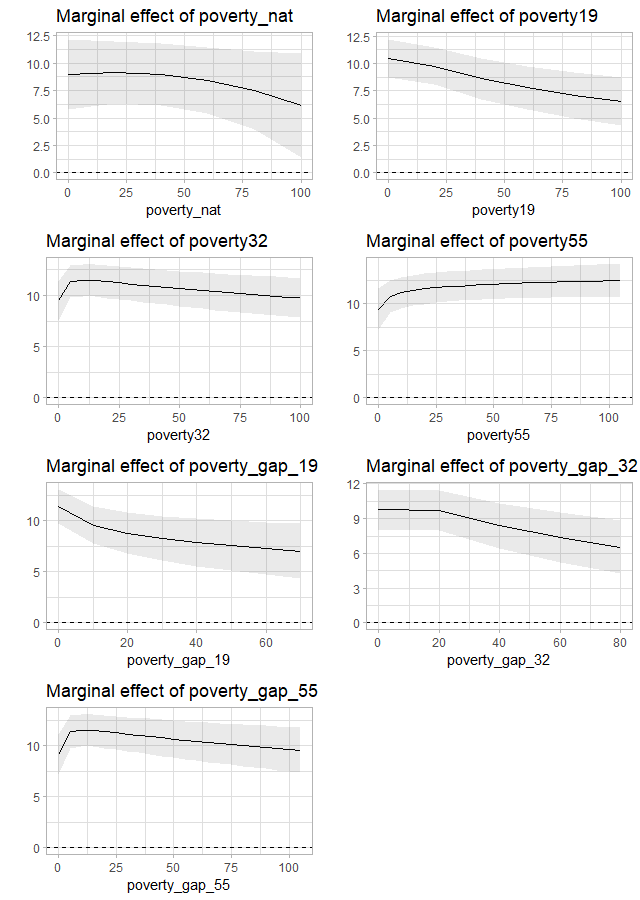
\includegraphics[width=\textwidth]{img/h2o_m.png}
    \caption{hypothesis 2, one-way fixed effects, margin effects}
    \label{h2o_m}
\end{figure}

\begin{figure}[h!]
    \centering
    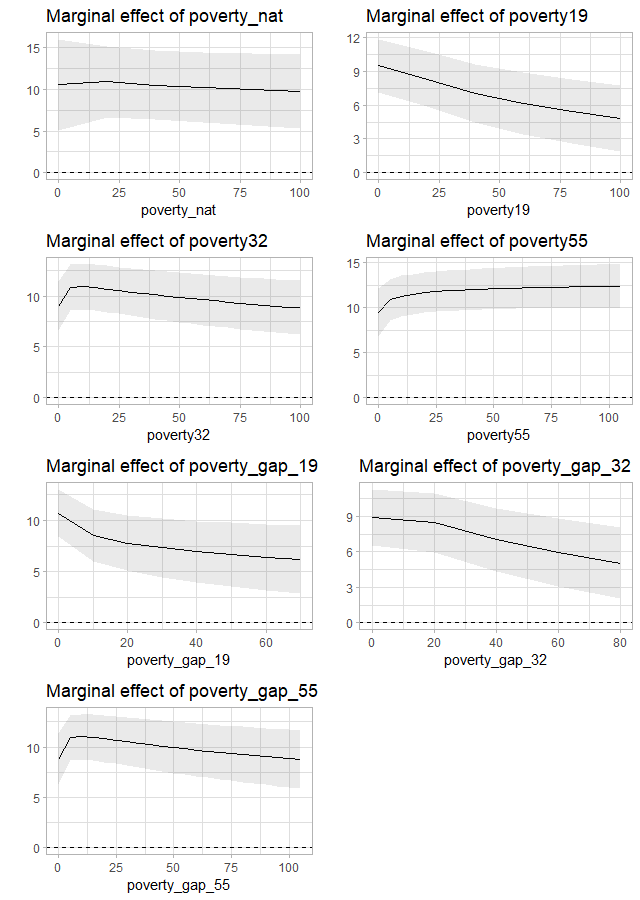
\includegraphics[width=\textwidth]{img/h2t_m.png}
    \caption{hypothesis 2, two-ways fixed effects, margin effects}
    \label{h2t_m}
\end{figure}


\begin{table}[!htbp] \centering 
  \caption{Hypothesis 3, individual fixed-effects} 
  \label{h3o} 
  \resizebox{\columnwidth}{!}{%
\begin{tabular}{@{\extracolsep{5pt}}lccccccc} 
\\[-1.8ex]\hline 
\hline \\[-1.8ex] 
 & \multicolumn{7}{c}{\textit{Dependent variable:}} \\ 
\cline{2-8} 
\\[-1.8ex] & \multicolumn{7}{c}{polity2\_lag} \\ 
\\[-1.8ex] & (1) & (2) & (3) & (4) & (5) & (6) & (7)\\ 
\hline \\[-1.8ex] 
 poverty\_nat & $-$0.205$^{*}$ &  &  &  &  &  &  \\ 
  & (0.112) &  &  &  &  &  &  \\ 
  & & & & & & & \\ 
 log(poverty19 + 1) &  & $-$5.224$^{*}$ &  &  &  &  &  \\ 
  &  & (2.829) &  &  &  &  &  \\ 
  & & & & & & & \\ 
 log(poverty32 + 1) &  &  & $-$4.635$^{*}$ &  &  &  &  \\ 
  &  &  & (2.470) &  &  &  &  \\ 
  & & & & & & & \\ 
 log(poverty55 + 1) &  &  &  & $-$3.903 &  &  &  \\ 
  &  &  &  & (2.614) &  &  &  \\ 
  & & & & & & & \\ 
 log(poverty\_gap\_19 + 1) &  &  &  &  & $-$7.060$^{*}$ &  &  \\ 
  &  &  &  &  & (3.967) &  &  \\ 
  & & & & & & & \\ 
 log(poverty\_gap\_32 + 1) &  &  &  &  &  & $-$5.108$^{*}$ &  \\ 
  &  &  &  &  &  & (3.015) &  \\ 
  & & & & & & & \\ 
 log(poverty\_gap\_55 + 1) &  &  &  &  &  &  & $-$4.184 \\ 
  &  &  &  &  &  &  & (2.627) \\ 
  & & & & & & & \\ 
 log(GDP\_pc\_ppp) & $-$0.444 & $-$0.510 & 0.455 & 0.730 & $-$0.649 & $-$0.249 & 0.487 \\ 
  & (0.550) & (0.408) & (0.422) & (0.484) & (0.425) & (0.389) & (0.424) \\ 
  & & & & & & & \\ 
 log(population\_WB) & 4.154$^{**}$ & 5.237$^{***}$ & 4.907$^{***}$ & 4.254$^{***}$ & 4.745$^{***}$ & 5.238$^{***}$ & 4.786$^{***}$ \\ 
  & (1.847) & (1.617) & (1.590) & (1.563) & (1.607) & (1.616) & (1.595) \\ 
  & & & & & & & \\ 
 v2regsupgroupssize & 1.719$^{***}$ & 1.840$^{***}$ & 1.876$^{***}$ & 1.851$^{***}$ & 1.791$^{***}$ & 1.870$^{***}$ & 1.869$^{***}$ \\ 
  & (0.519) & (0.604) & (0.653) & (0.646) & (0.567) & (0.627) & (0.652) \\ 
  & & & & & & & \\ 
 v2xeg\_eqdr & 7.925$^{**}$ & 5.394 & 4.935 & 4.554 & 5.056 & 5.285 & 4.828 \\ 
  & (3.400) & (3.918) & (3.693) & (3.726) & (3.896) & (3.893) & (3.741) \\ 
  & & & & & & & \\ 
 log(gini\_WB) & $-$2.766 & $-$2.599 & $-$5.839$^{**}$ & $-$6.681$^{**}$ & $-$1.856 & $-$3.174 & $-$5.481$^{**}$ \\ 
  & (2.166) & (1.970) & (2.308) & (2.644) & (1.934) & (1.963) & (2.289) \\ 
  & & & & & & & \\ 
 poverty\_nat:log(gini\_WB) & 0.054$^{*}$ &  &  &  &  &  &  \\ 
  & (0.030) &  &  &  &  &  &  \\ 
  & & & & & & & \\ 
 log(poverty19 + 1):log(gini\_WB) &  & 1.310$^{*}$ &  &  &  &  &  \\ 
  &  & (0.736) &  &  &  &  &  \\ 
  & & & & & & & \\ 
 log(poverty32 + 1):log(gini\_WB) &  &  & 1.419$^{**}$ &  &  &  &  \\ 
  &  &  & (0.712) &  &  &  &  \\ 
  & & & & & & & \\ 
 log(poverty55 + 1):log(gini\_WB) &  &  &  & 1.328$^{*}$ &  &  &  \\ 
  &  &  &  & (0.787) &  &  &  \\ 
  & & & & & & & \\ 
 log(poverty\_gap\_19 + 1):log(gini\_WB) &  &  &  &  & 1.681$^{*}$ &  &  \\ 
  &  &  &  &  & (1.005) &  &  \\ 
  & & & & & & & \\ 
 log(poverty\_gap\_32 + 1):log(gini\_WB) &  &  &  &  &  & 1.348$^{*}$ &  \\ 
  &  &  &  &  &  & (0.788) &  \\ 
  & & & & & & & \\ 
 log(poverty\_gap\_55 + 1):log(gini\_WB) &  &  &  &  &  &  & 1.318$^{*}$ \\ 
  &  &  &  &  &  &  & (0.754) \\ 
  & & & & & & & \\ 
\hline \\[-1.8ex] 
Observations & 651 & 1,412 & 1,412 & 1,412 & 1,412 & 1,412 & 1,412 \\ 
R$^{2}$ & 0.155 & 0.199 & 0.194 & 0.196 & 0.208 & 0.192 & 0.192 \\ 
Adjusted R$^{2}$ & $-$0.035 & 0.103 & 0.097 & 0.100 & 0.113 & 0.095 & 0.095 \\ 
F Statistic & 13.903$^{***}$ (df = 7; 531) & 44.839$^{***}$ (df = 7; 1260) & 43.337$^{***}$ (df = 7; 1260) & 43.882$^{***}$ (df = 7; 1260) & 47.352$^{***}$ (df = 7; 1260) & 42.744$^{***}$ (df = 7; 1260) & 42.702$^{***}$ (df = 7; 1260) \\ 
\hline 
\hline \\[-1.8ex] 
\textit{Note:}  & \multicolumn{7}{r}{$^{*}$p$<$0.1; $^{**}$p$<$0.05; $^{***}$p$<$0.01} \\ 
\textit{Note: all the models use robust standard errors}  & \multicolumn{7}{r}{$^{*}$p$<$0.1; $^{**}$p$<$0.05; $^{***}$p$<$0.01} \\ 
\end{tabular} 
}
\end{table} 

\begin{figure}[h!]
    \centering
    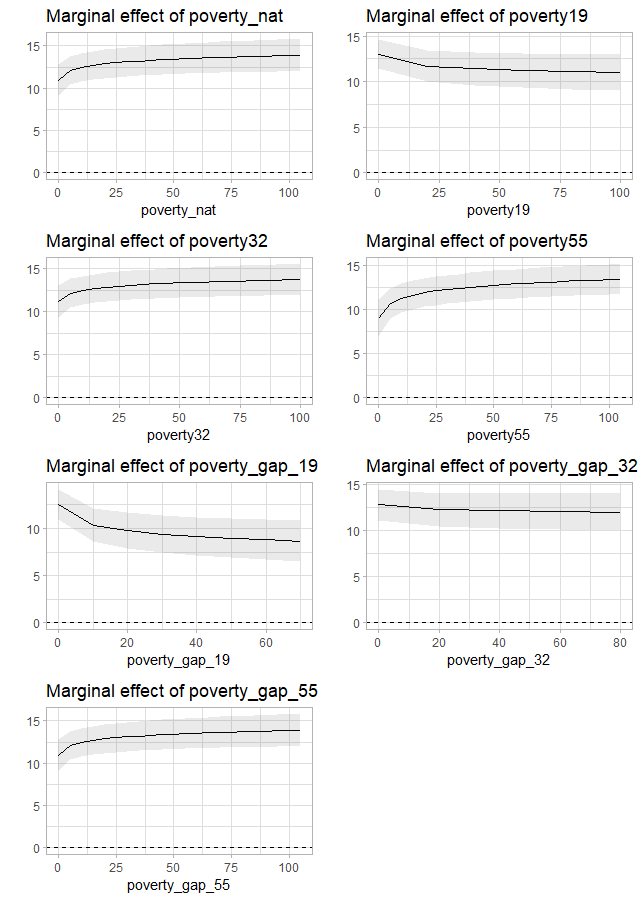
\includegraphics[width=\textwidth]{img/h3o_m.png}
    \caption{hypothesis 3, one-way fixed effects, margin effects}
    \label{h3o_m}
\end{figure}

\begin{figure}[h!]
    \centering
    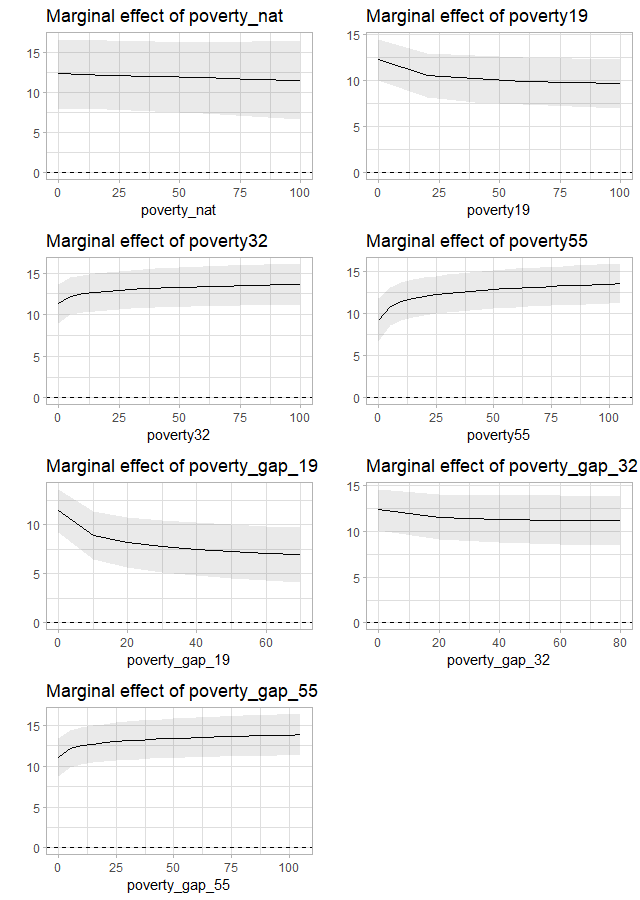
\includegraphics[width=\textwidth]{img/h3t_m.png}
    \caption{hypothesis 3, two-ways fixed effects, margin effects}
    \label{h3t_m}
\end{figure}

\begin{table}[!htbp] \centering 
  \caption{Robust check, hypothesis 2, individual fixed effects} 
  \label{r2o} 
  \resizebox{\columnwidth}{!}{%
\begin{tabular}{@{\extracolsep{5pt}}lccccccc} 
\\[-1.8ex]\hline 
\hline \\[-1.8ex] 
 & \multicolumn{7}{c}{\textit{Dependent variable:}} \\ 
\cline{2-8} 
\\[-1.8ex] & \multicolumn{7}{c}{regime\_lag} \\ 
\\[-1.8ex] & (1) & (2) & (3) & (4) & (5) & (6) & (7)\\ 
\hline \\[-1.8ex] 
 poverty\_nat & 0.019 &  &  &  &  &  &  \\ 
  & (0.039) &  &  &  &  &  &  \\ 
  & & & & & & & \\ 
 I(poverty\_nat$\hat{\mkern6mu}$2) & $-$0.0005 &  &  &  &  &  &  \\ 
  & (0.0005) &  &  &  &  &  &  \\ 
  & & & & & & & \\ 
 log(poverty19 + 1) &  & $-$0.252 &  &  &  &  &  \\ 
  &  & (0.237) &  &  &  &  &  \\ 
  & & & & & & & \\ 
 I((poverty19 + 1)$\hat{\mkern6mu}$2) &  & $-$0.0004 &  &  &  &  &  \\ 
  &  & (0.0002) &  &  &  &  &  \\ 
  & & & & & & & \\ 
 log(poverty32 + 1) &  &  & 1.180$^{**}$ &  &  &  &  \\ 
  &  &  & (0.504) &  &  &  &  \\ 
  & & & & & & & \\ 
 I(log(poverty32 + 1)$\hat{\mkern6mu}$2) &  &  & $-$0.243$^{**}$ &  &  &  &  \\ 
  &  &  & (0.107) &  &  &  &  \\ 
  & & & & & & & \\ 
 log(poverty55 + 1) &  &  &  & 0.623 &  &  &  \\ 
  &  &  &  & (0.453) &  &  &  \\ 
  & & & & & & & \\ 
 I(log(poverty55 + 1)$\hat{\mkern6mu}$2) &  &  &  & $-$0.031 &  &  &  \\ 
  &  &  &  & (0.109) &  &  &  \\ 
  & & & & & & & \\ 
 log(poverty\_gap\_19 + 1) &  &  &  &  & $-$0.280 &  &  \\ 
  &  &  &  &  & (0.419) &  &  \\ 
  & & & & & & & \\ 
 I(log(poverty\_gap\_19 + 1)$\hat{\mkern6mu}$2) &  &  &  &  & $-$0.111 &  &  \\ 
  &  &  &  &  & (0.149) &  &  \\ 
  & & & & & & & \\ 
 log(poverty\_gap\_32 + 1) &  &  &  &  &  & 1.126$^{**}$ &  \\ 
  &  &  &  &  &  & (0.554) &  \\ 
  & & & & & & & \\ 
 I(log(poverty\_gap\_32 + 1)$\hat{\mkern6mu}$2) &  &  &  &  &  & $-$0.372$^{**}$ &  \\ 
  &  &  &  &  &  & (0.161) &  \\ 
  & & & & & & & \\ 
 log(poverty\_gap\_55 + 1) &  &  &  &  &  &  & 1.367$^{**}$ \\ 
  &  &  &  &  &  &  & (0.537) \\ 
  & & & & & & & \\ 
 I(log(poverty\_gap\_55 + 1)$\hat{\mkern6mu}$2) &  &  &  &  &  &  & $-$0.279$^{**}$ \\ 
  &  &  &  &  &  &  & (0.129) \\ 
  & & & & & & & \\ 
 log(GDP\_pc\_ppp) & $-$0.222 & $-$0.255 & 0.177 & 0.426 & $-$0.259 & 0.021 & 0.212 \\ 
  & (0.401) & (0.286) & (0.281) & (0.311) & (0.283) & (0.259) & (0.285) \\ 
  & & & & & & & \\ 
 log(population\_WB) & 1.653 & 2.292$^{**}$ & 2.185$^{**}$ & 2.412$^{**}$ & 2.311$^{**}$ & 1.960$^{*}$ & 2.180$^{**}$ \\ 
  & (1.073) & (1.091) & (1.031) & (1.016) & (1.073) & (1.058) & (1.019) \\ 
  & & & & & & & \\ 
 v2regsupgroupssize & 1.064$^{***}$ & 1.117$^{***}$ & 1.148$^{***}$ & 1.170$^{***}$ & 1.134$^{***}$ & 1.123$^{***}$ & 1.159$^{***}$ \\ 
  & (0.389) & (0.386) & (0.411) & (0.438) & (0.391) & (0.389) & (0.417) \\ 
  & & & & & & & \\ 
 v2xeg\_eqdr & 5.903$^{***}$ & 3.931 & 3.562 & 3.672 & 3.781 & 3.564 & 3.664 \\ 
  & (2.205) & (2.680) & (2.683) & (2.657) & (2.734) & (2.649) & (2.689) \\ 
  & & & & & & & \\ 
 log(gini\_WB) & $-$0.084 & 0.324 & $-$0.952 & $-$1.081 & 0.584 & $-$0.506 & $-$0.834 \\ 
  & (1.286) & (1.133) & (1.161) & (1.153) & (1.242) & (1.082) & (1.196) \\ 
  & & & & & & & \\ 
\hline \\[-1.8ex] 
Observations & 651 & 1,412 & 1,412 & 1,412 & 1,412 & 1,412 & 1,412 \\ 
R$^{2}$ & 0.133 & 0.193 & 0.194 & 0.180 & 0.190 & 0.203 & 0.191 \\ 
Adjusted R$^{2}$ & $-$0.061 & 0.096 & 0.097 & 0.082 & 0.093 & 0.108 & 0.094 \\ 
F Statistic & 11.663$^{***}$ (df = 7; 531) & 42.951$^{***}$ (df = 7; 1260) & 43.296$^{***}$ (df = 7; 1260) & 39.485$^{***}$ (df = 7; 1260) & 42.314$^{***}$ (df = 7; 1260) & 45.946$^{***}$ (df = 7; 1260) & 42.375$^{***}$ (df = 7; 1260) \\ 
\hline 
\hline \\[-1.8ex] 
\textit{Note: all the models use robust standard errors}  & \multicolumn{7}{r}{$^{*}$p$<$0.1; $^{**}$p$<$0.05; $^{***}$p$<$0.01} \\ 
\end{tabular} 
}
\end{table} 



\begin{figure}[h!]
    \centering
    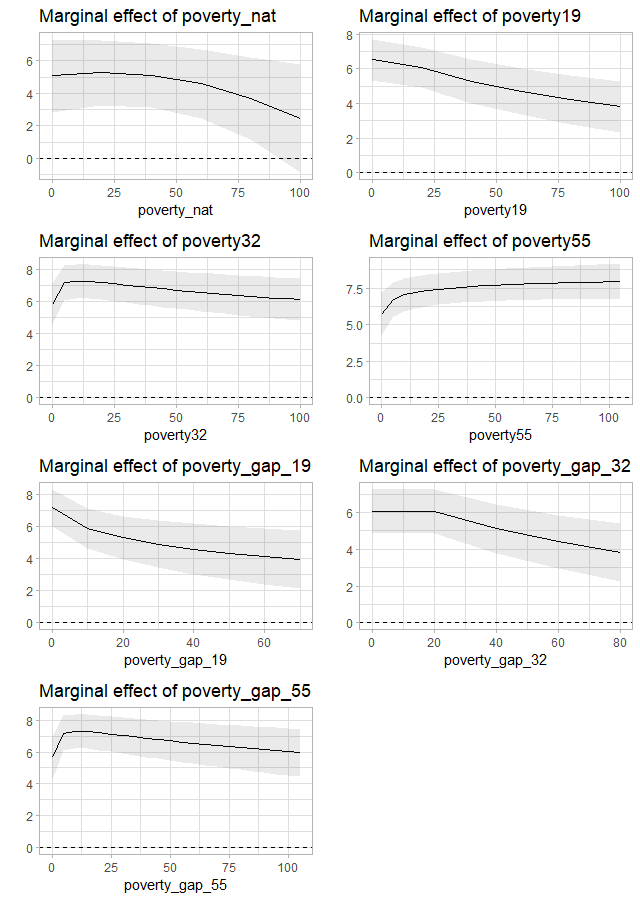
\includegraphics[width=\textwidth]{img/r2o_m.png}
    \caption{Robust check, hypothesis 2, one-way fixed effects, margin effects}
    \label{r2o_m}
\end{figure}

\begin{figure}[h!]
    \centering
    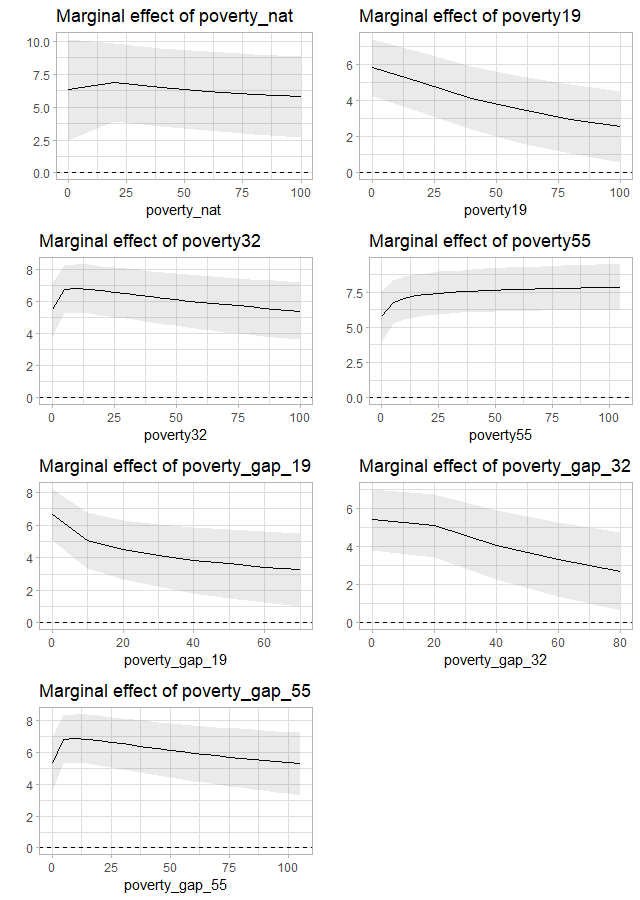
\includegraphics[width=\textwidth]{img/r2t_m.png}
    \caption{Robust check, hypothesis 2, two-ways fixed effects, margin effects}
    \label{r2t_m}
\end{figure}



\end{document}
